\documentclass[12pt, a4paper]{article} % 10pt font size (11 and 12 also possible), A4 paper (letterpaper for US letter) and two column layout (remove for one column)

%----------------------------------------------------------------------------------------
%	PACKAGES AND OTHER DOCUMENT CONFIGURATIONS
%----------------------------------------------------------------------------------------

\usepackage[ngerman]{babel}

\usepackage[hang,small,labelfont=bf,up,textfont=it]{caption} % Custom captions under/above tables and figures

\usepackage{booktabs} % Horizontal rules in tables

\usepackage{graphicx} % Required for adding images
\graphicspath{{figure/}}

\usepackage{enumitem} % Required for customising lists
\setlist{noitemsep} % Remove spacing between bullet/numbered list elements

\usepackage[hidelinks]{hyperref}

\usepackage{tabularx}

\usepackage[verbose]{placeins}

\usepackage[official]{eurosym}

\usepackage{longtable}

\urlstyle{same}

\pretolerance=8000
\tolerance=5000
\emergencystretch=10pt % https://tex.stackexchange.com/questions/31301/how-to-reduce-the-number-of-hyphenation
\usepackage{indentfirst}

\usepackage[autostyle=true]{csquotes} % Required to generate language-dependent quotes in the bibliography

%----------------------------------------------------------------------------------------
%	MARGINS AND SPACING
%----------------------------------------------------------------------------------------

\usepackage{geometry} % Required for adjusting page dimensions
\usepackage{changepage}
\usepackage{calc}

\geometry{
    head=1cm,
    foot=3cm,
    top=2cm, % Top margin
    bottom=0cm, % Bottom margin
    left=3cm, % Left margin
    right=3cm, % Right margin
    includehead, % Include space for a header
    includefoot, % Include space for a footer
    %showframe, % Uncomment to show how the type block is set on the page
}

\setlength{\columnsep}{7mm} % Column separation width

%----------------------------------------------------------------------------------------
%	FONTS
%----------------------------------------------------------------------------------------

\usepackage[utf8]{inputenc} % Required for inputting international characters
\usepackage[T1]{fontenc}
\usepackage[default,scale=0.95]{opensans}
\usepackage{eurosym}

%----------------------------------------------------------------------------------------
%   TOC
%----------------------------------------------------------------------------------------
\setcounter{tocdepth}{2}

%----------------------------------------------------------------------------------------
%	HEADERS AND FOOTERS
%----------------------------------------------------------------------------------------

\usepackage{fancyhdr} % Needed to define custom headers/footers
\pagestyle{fancy} % Enables the custom headers/footers

\lhead{} % Left header

%----------------------------------------------------------------------------------------
%	TITLE SECTION
%----------------------------------------------------------------------------------------

\usepackage{titling} % Allows custom title configuration

\newcommand{\HorRule}{\rule{\linewidth}{1pt}} % Defines the horizontal rule around the title

\pretitle{
    \vspace{60pt} % Move the entire title section up
    \hspace{310pt}
    \\
    \\
    \vspace{40pt}
    \HorRule\vspace{10pt} % Horizontal rule before the title
    \centering\Huge\textbf
}

\posttitle{\par\vskip 15pt} % Whitespace under the title

\preauthor{} % Anything that will appear before \author is printed

\postauthor{ % Anything that will appear after \author is printed
    \vspace{10pt} % Space before the rule
    \par\HorRule % Horizontal rule after the title
    \vspace{150pt} % Space after the title section
}

\usepackage{xcolor}
\definecolor{df}{HTML}{b5dc17}
\usepackage{tikz}

\usepackage{eso-pic}
\newcommand\BackgroundPic{%
    \put(0,0){%
        \parbox[b][\paperheight]{\paperwidth}{%
            
\includegraphics[width=\paperwidth,height=\paperheight,keepaspectratio]{title_background.pdf}%
        }
    }
}


\fancyfootoffset[L]{\dimexpr\oddsidemargin+1in\relax}
\newcommand*\rect[1]{\begin{tikzpicture}[remember picture,overlay]\fill[df] (0,0) rectangle
        (\paperwidth,\headheight);\node at (0,0.5) {#1};\end{tikzpicture}}

\fancyfoot[L]{\rect{}}
\fancyfoot[C]{\rect{}}
\fancyfoot[R]{\rect{\thepage}}

 % Specifies the document structure and loads requires packages

\renewcommand\thepart{\Alph{part}}

%----------------------------------------------------------------------------------------
%	ARTICLE INFORMATION
%----------------------------------------------------------------------------------------

\begin{document}

\title{
Tür an Tür - Digital Factory gGmbH\\
Wirkungsbericht 2018\\
} % The article title

\AddToShipoutPicture*{\BackgroundPic}

\date{}

\maketitle
\thispagestyle{empty} % Disables header on first page (must be after \maketitle)

%----------------------------------------------------------------------------------------
%	ABSTRACT
%----------------------------------------------------------------------------------------

%----------------------------------------------------------------------------------------
%	ARTICLE CONTENTS
%----------------------------------------------------------------------------------------

\newpage
\tableofcontents

\newpage

\hypertarget{vorwort}{%
\section{Vorwort}\label{vorwort}}

Lieber Förderer, liebe Partner, liebe Wegbegleiterinnen und Wegbegleiter
von Integreat und der Digitalfabrik,
\\

dies ist nun der dritte Wirkungsbericht der Tür an Tür – Digital Factory
gGmbH (kurz: Digitalfabrik). Allein diese Tatsache zeigt, wie sich die
Arbeit des Teams aus dem Ad-Hoc-Projekt zu sehr großer Kontinuität
gewandelt hat, aber auch, wie wichtig uns von Anfang an das Thema
Wirkung gewesen ist. Für die Kontinuität des Projekts gibt es viele
weitere Beispiele. So traf sich das Integreat-Team Ende des Jahres 2018
bereits zum 13. Mal zur Integreat-Konferenz an der Informatik-Fakultät
der TU-München mit einer über die Jahre sehr konstanten
Teilnehmer*innenzahl. Personell gab es wenige Änderungen im letzten
Jahr, was von einer hohen und langanhaltenden Motivation der
Ehrenamtlichen zeugt. Die Anzahl der kooperierenden Kommunen wuchs über
das Jahr weiter und ermöglicht dem Projekt insgesamt eine immer
langfristigere Perspektive.

Es gab aber natürlich auch viele Veränderungen. Wir beschlossen, weitere
hauptamtliche Stellen bei der Digitalfabrik einzurichten, um sowohl die
langfristige Wirksamkeit von bestehenden Projekten zu sichern, als auch
neue Pfade außerhalb der bisher existierenden Projekte zu beschreiten.
Technologisch hat sich das Team dafür entschieden, die Zöpfe, die
anfangs sehr hastig geflochten wurden, abzuschneiden und durch auf
langfristigen Betrieb angelegte Lösungen zu ersetzen. Diese Aufgabe wird
uns über große Teile des Jahres 2019 beschäftigen.

Ebenfalls stark verändert hat sich die Einstellung des Teams. Während
anfangs der Fokus auf möglichst zeitnah erreichbaren Zielen und
dementsprechend pragmatischen Ansätzen und Lösungen lag, gelangen nun
Nachhaltigkeit und Langfristigkeit zunehmend in den Fokus. Es bleibt uns
aber nach wie vor wichtig, die Digitalfabrik als Raum für spontane Ideen
und dynamische Entwicklungen zu erhalten. Im Jahr 2018 verstärkten wir
auch unsere Bemühungen um internationale Vernetzung und Kooperationen.
Sehr spannend für uns war die überaus positive Rezeption, die das
Integreat-Projekt international erfährt. Von vielen Organisationen wird
Integreat als Vorbild für ein nachhaltiges und gemeinnütziges IT-Projekt
wahrgenommen. All dies zeigt, mit wie viel Rückenwind sowohl die
Digitalfabrik als auch das Integreat-Projekt in das Jahr 2019 starten.
Die Ergebnisse des kommenden Jahres werden wir selbstverständlich im
nächsten Wirkungsbericht wiederfinden.


\includegraphics[width=2.0197in,height=0.95764in]{./media/image1.png}

Sven Seeberg-Elverfeldt

Technischer Koordinator

\hypertarget{einleitung}{%
\section{Einleitung}\label{einleitung}}

\hypertarget{vision-und-ansatz}{%
\subsection{Vision und Ansatz}\label{vision-und-ansatz}}

Die Tür an Tür - Digital Factory gGmbH (im Folgenden weiterhin
Digitalfabrik genannt) wurde im Juni 2016 mit dem Ziel gegründet,
Geflüchteten den Einstieg in die neue Gesellschaft zu erleichtern.
Dieses Vorhaben wurde von Beginn an in Zusammenarbeit mit etablierten
und erfahrenen Organisationen und Institutionen sowie kommunalen
Verwaltungen verfolgt. Das starke Netzwerk, das die Digitalfabrik seit
den Anfängen des Projekts Integreat im Jahr 2015 begleitet, ist seitdem
wichtigste Voraussetzung für die sich entfaltende Wirkung der
Organisation. Netzwerke aufzubauen und Synergiepotentiale zu
identifizieren und nutzbar zu machen, sind zum elementaren Teil der
organisationalen Arbeit geworden. Insbesondere in der intrakommunalen
und interkommunalen Zusammenarbeit konnten bereits Erfolge festgestellt
werden. Darunter verstehen wir die Zusammenarbeit von Akteuren innerhalb
einer Kommune (intrakommunal) und kommunenübergreifend (interkommunal).
Auch weiterhin soll dazu beitragen werden, dass die Netzwerke in diesen
beiden Bereich gestärkt werden und die vorhandenen Ressourcen in der
Integrationsarbeit somit effektiv eingesetzt werden können.

Die Vision, die wir mit unserer Arbeit verfolgen und deren
Verwirklichung als Maßstab für alle Aktivitäten der Organisation
auftritt, ist es, Informationen für alle Menschen verständlich,
zugänglich und verarbeitbar („accessible“) zu machen. Die
Marginalisierung von Menschen aus anderen Ländern und Kulturen in der
Gesellschaft ist laut aktuellen Forschungen oft auf Informationsarmut
begründet. Der Abbau von Informationsarmut durch Lösungen wie Integreat
und die damit gewonnene Gleichberechtigung im Informationszugang stellen
wichtige Meilensteine für die Entwicklung zu einer freien Gesellschaft
dar. Langfristig sind unsere Angebote – insbesondere die
Informations-App Integreat – darauf ausgelegt nicht nur Geflüchteten bei
der Orientierung und Informationsgewinnung zu unterstützen, sondern für
alle Neuzugewanderten und Bürgerinnen und Bürger als hilfreiche Stütze
im Alltag und als Kommunikationskanal zur lokalen Verwaltung zu dienen.
Wie der Name bereits impliziert, will die Digitalfabrik digitale Brücken
bauen, um die lokale Integrationsarbeit zu stärken, ohne sie ersetzen zu
wollen.

Um diesen Fortschritt zu unterstützen und gleichzeitig das übergeordnete
Ziel von gemeinschaftlicher Entwicklung und Nutzung von Inhalten und
Software zu verfolgen, setzen wir in unserer Arbeit auf Open Source
Technologien und verwenden Creative Commons Lizenzen. So senken wir
Hemmschwellen und technische Barrieren ab, um die oben beschriebene
Zusammenarbeit initial zu befähigen, zu stärken und langfristig zu
etablieren. Frei nach dem Ansatz „Learning by Doing“ werden öffentliche
Verwaltungen durch Ansätze von uns an die Vorteile und Chancen, die
offen verfügbare Inhalte und Software bieten, herangeführt und können
diese in der eigenen Arbeit direkt erfahren. Können Erfolge der Arbeit
mit gemeinschaftlich erarbeiteter und offener Software und Inhalten
unter freier Lizenz in einem Bereich der Verwaltung – in diesem Fall der
Integrationsarbeit – verzeichnet werden, entwickeln sich Transfermodelle
und die Übernahme von Ansätzen und Methoden auch in andere Bereiche
innerhalb der Kommune. Wenn öffentliche Gelder in die Entwicklung von
Software oder von Inhalten investiert werden, sollten diese auch der
Öffentlichkeit zur Verfügung stehen. Davon sind wir überzeugt und wollen
mit unserer Arbeit gezielt zu dem entsprechenden Systemwandel beitragen.

\hypertarget{gegenstand-dieses-berichts}{%
\subsection{Gegenstand dieses
Berichts}\label{gegenstand-dieses-berichts}}

\begin{tabularx}{\textwidth}{p{4cm}X}
\toprule
Geltungsbereich & Dieser Bericht bezieht sich auf die Aktivitäten der
Tür an Tür - Digital Factory gGmbH. Ein besonderer Fokus wird auf das
zentrale Angebot von Integreat gelegt.\tabularnewline
\midrule
Berichtzeitraum und Berichtzyklus & Wir berichten über unsere Arbeit im
Jahr 2018. Die Digitalfabrik veröffentlicht einmal im Jahr einen
Wirkungsbericht.\tabularnewline
\midrule
Anwendung des SRS & In diesem Bericht orientieren wir uns an den
Vorgaben der aktuellen Version des Social Reporting Standards (SRS),
Stand 2014. Dies ist der dritte Jahresbericht nach dem
SRS.\tabularnewline
\midrule
Ansprechpartnerin & \begin{minipage}[t]{\columnwidth}
Clara Bracklo

bracklo@integreat-app.de\end{minipage}\tabularnewline

\bottomrule
\end{tabularx}

\hypertarget{die-gesellschaftliche-herausforderung-und-der-luxf6sungsansatz}{%
\section{Die gesellschaftliche Herausforderung und der
Lösungsansatz}\label{die-gesellschaftliche-herausforderung-und-der-luxf6sungsansatz}}

\hypertarget{die-gesellschaftliche-herausforderung}{%
\subsection{Die gesellschaftliche
Herausforderung}\label{die-gesellschaftliche-herausforderung}}

Über 68 Millionen Menschen sind derzeit weltweit auf der Flucht.
Schätzungen zufolge suchen 40 Millionen von ihnen als Binnenflüchtlinge
Schutz m eigenen Land . Einem Großteil wurde allerdings durch Kriege und
Verfolgung die Sicherheit in der Heimat genommen und diese Menschen sind
gezwungen das Heimatland zu verlassen und in einem fremden Land Schutz
zu suchen. Die Herausforderungen, die sich dadurch für Organisationen,
Länder und Kommunen ergeben, sind auch in Europa und in Deutschland zu
spüren.

Zuwanderung allein stellt jedoch keine tatsächlich neue Entwicklung in
Deutschland dar. Die Bundesrepublik hat in der Vergangenheit gezielt
Arbeitsmigration gefördert und hat somit eine lange Geschichte als
Einwanderungsland. Trotz verschiedener Migrations- und Fluchtbewegungen
in der Vergangenheit, erhielt diese Lage durch starke mediale Präsenz
und die politische Debatte wie bereits auch Anfang der 90er Jahre und
erneutseit 2015 besondere gesellschaftliche Aufmerksamkeit.

Im Vergleich zu früheren Migrationsbewegung nach Deutschland, spielen
digitale Technologien für die Neuzugewanderten heute eine weitaus
bedeutendere Rolle, wie wir es auch in anderen Bereichen beobachten
können. Der Gebrauch von Smartphones ist quer durch die Gesellschaft
nahezu unabhängig von Altersstruktur und kulturellem Hintergrund zur
Informationsbeschaffung üblich. Auf der Flucht dient das Smartphone der
Kontaktaufnahme mit der Familie, als Navigator und der generellen
Informationsbeschaffung. Nach der Ankunft wird das Smartphone zur
Orientierung und als Kommunikationskanal genutzt und ist als wichtiges
Medium zur Integration zu verstehen. Diesen Zugang jedoch effektiv zu
nutzen und beispielsweise Informationsangebote und Vernetzung
anzubieten, ist insbesondere für kommunale Verwaltungen, die bereits mit
bestehenden Aufgaben stark ausgelastet sind, nahezu unmöglich.
Gemeinsame digitale Kommunikationsräume existieren nicht. Einen
gemeinsamen Kommunikationsraum zu schaffen, der die Verwaltungen,
Organisationen und Neuzugewanderten gleichermaßen erreicht ist daher
besonders wichtig, um die Integrationsarbeit vor Ort langfristig zu
verbessern und nach Möglichkeit zu entlasten.

Über die letzten vier Jahre, in denen die Digitalfabrik bereits aktiv im
Bereich der Integrationsarbeit tätig ist, konnten wir auf kommunaler
Ebene ein wachsendes Bewusstsein für die Bedarfe an Informationen und
Kommunikation verschiedener Migrantengruppen – insbesondere aus anderen
europäischen Ländern – feststellen. Dass Hilfsangebote sich nicht nur
auf einzelne Gruppen aus der tagespolitischen Diskussion richten sollten
und dürfen ist ein Anliegen unserer kommunalen Partner und auch der
Digitalfabrik selbst. Integrationsangebote für möglichst viele Menschen
zugänglich zu machen, sichert die Langfristigkeit der Projekte und kann
die Wirkung der Aktivitäten ausweiten und verstärken.

Neben den wichtigen gesellschaftlichen Entwicklungen aus dem Bereich der
Integration und Zuwanderung ist abschließend die aktuelle öffentliche
Debatte zur Verwendung und Entwicklung freier Software (Open Source
Software) in der Verwaltung zu nennen. Die Forderung verschiedener
Organisationen lässt sich folgendermaßen zusammenfassen: Werden
öffentliche Gelder (Steuergelder) zur Entwicklung oder Nutzung von
Software eingesetzt, so soll die Software selbst ebenfalls öffentlich
und frei zugänglich sein und nicht von einzelnen Unternehmen unter
Verschluss gehalten werden. Der Systemwandel, der zur Verwirklichung
dieser Forderung notwendig ist, ist komplex und muss viele alte
Strukturen aufbrechen. Die damit einhergehende Herausforderung ist somit
nicht zu unterschätzen.

\hypertarget{die-angebotslandschaft}{%
\subsection{Die Angebotslandschaft}\label{die-angebotslandschaft}}

Neben der persönlichen Beratung, die auch unserer Meinung immer
zentraler Bestandteil des Integrationsprozesses sein sollte und sein
muss, haben Kommunen die Bekanntmachung von lokalen Informationen und
Angeboten in der Vergangenheit vor allem durch das Verfassen und
aufwendige Drucken sowie Verteilen von Printmaterialien forciert. Waren
die Printmaterialien einmal gedruckt, ließen sich die Inhalte nur mit
großer zeitlicher Verzögerung und viel Aufwand aktualisieren.
Entsprechendes Informationsmaterial war häufig nur in deutscher Sprache
verfügbar, da Übersetzungen nicht nur teuer, sondern auch durch die
Herstellung zu aufwendig für viele Kommunen waren.

Digitale Technologien stellen einen geeigneten Weg zur Vermittlung von
Informationen an neuzugewanderte Menschen dar, da Mehrsprachigkeit
leichter und kostengünstiger umsetzbar und der Zugang lokal ungebunden
ist. Somit stellen entsprechende Technologien eine leicht
aktualisierbare und gut zugängliche Alternative zu herkömmlichen
Printmaterialien dar. Diese Erkenntnis motivierte verschiedene
etablierte und auch neue Unternehmen und Organisationen zur Entwicklung
von entsprechenden Lösungsansätzen.

In der Gründungszeit der Digitalfabrik Mitte 2016 entstanden somit neben
der hauseigenen Informations-App Integreat auch andere
Informationsportale von verschiedenen Anbietern. Zu nennen sind an
dieser Stelle unter anderem die Ankommen-App des BAMF, die App Moin
Refugee, die Welcome App Germany und die App Welcome to NRW als Angebote
in Deutschland. Gemeinsam ist diesen Angeboten und der Integreat-App die
grundsätzliche Darstellung von Informationen für Neuzugewanderte. Trotz
bestimmter Überschneidungen ist über zwei Jahre nach der besonders
starken Zuwanderung 2015 auffällig, dass die Angebote mit Ausnahme der
Integreat-App nur noch partiell oder gar nicht mehr weiterentwickelt
werden.

\hypertarget{die-positionierung-der-tuxfcr-an-tuxfcr-digital-factory-ggmbh}{%
\subsection{Die Positionierung der Tür an Tür – Digital Factory
gGmbH}\label{die-positionierung-der-tuxfcr-an-tuxfcr-digital-factory-ggmbh}}

Um dieses Phänomen zu verstehen und gleichzeitig an die Wirkung der
Digitalfabrik heranzuführen, ist die Positionierung der Organisation in
dieser Angebotslandschaft besonders relevant. Bereits die
Entstehungsgeschichte der Organisation ist für den besonderen Charakter
beschreibend. So wurde die Organisation nicht um ihrer selbst wegen
gegründet, sondern war Ergebnis von organischem, bedarfsorientiertem
Wachstum.

Als im Jahr 2015 über eine Million Geflüchtete nach Deutschland kamen,
wurde der Bedarf an mehrsprachigen Informationsangeboten zu Asylthemen
und Alltagsfragen schnell deutlich. So auch in Augsburg, wo sich eine
Gruppe engagierter Studierender gemeinsam mit dem Tür an Tür -
miteinander wohnen und leben e.V. (Tür an Tür e.V.), der Stadt Augsburg
und dem Lehrstuhl für Wirtschaftsinformatik der TU München an die
Digitalisierung der 1997 erschienenen „First Steps“-Broschüre mit
lokalen Erstinformationen für Asylbewerberinnen und Asylbewerber in der
Region Augsburg machte. Als Ergebnis entstand im Sommer 2015 die
Integreat-App als digitaler Alltagsguide für Geflüchtete, die in
Augsburg im November 2015 offiziell vom Bürgermeister vorgestellt wurde.
Nach der Bekanntmachung der Integreat-App in und für Augsburg kamen auch
andere Kommunen und Landkreise auf das Team zu, die die Lösung für ihre
Region einsetzen wollten. Die Gründung der Tür an Tür – Digital Factory
gGmbH folgte ebenfalls aufgrund der direkten Anfrage und dem Bedarf der
kommunalen Partner die Zusammenarbeit an der Integreat-App professionell
zu gestalten und für Planungssicherheit zu sorgen.

Mittlerweile hat sich die Digitalfabrik zu einem Beratungs- und
Dienstleistungsunternehmen für verschiedene digitale Projekte im
sozialen und öffentlichen Bereich entwickelt. Die Erfahrungen und
Expertise, die durch die mehrjährige Zusammenarbeit mit Institutionen
aus beiden Bereichen gewonnen wurden, geben wir in unserer täglichen
Arbeit an unsere Partner und gleichgesinnte Organisationen weiter. Das
im Laufe dieser Zeit entstandene Netzwerk stellt eine wichtige Grundlage
für unsere Aktivitäten dar und ermöglicht es Ressourcen gemeinsam zu
nutzen und im nächsten Schritt auch anderen zugänglich zu machen.

Die Digitalfabrik versteht sich als Wegbereiter für die positive
Entwicklung und Öffnung von öffentlichen und sozialen Institutionen
durch Einsatz digitaler Lösungen. Dies unterstützen wir mit all unseren
Aktivitäten. Aufgrund der besonderen Relevanz und dem Einfluss auf die
wirkungsorientierte Arbeitsweise soll im Folgenden die App Integreat
genauer vorgestellt werden.

\hypertarget{die-besondere-rolle-der-app-integreat}{%
\subsection{Die besondere Rolle der App
Integreat}\label{die-besondere-rolle-der-app-integreat}}

Das Herzstück der Digitalfabrik ist die Informations-App Integreat.
Dieses Angebot – welches ursprünglich für Geflüchtete entwickelt wurde –
richtet sich heute konkret an Neuzugewanderte, die sich selbstständig in
ihrem neuen kommunalen Umfeld informieren und orientieren möchten.

Auf kommunaler Ebene ist der Bedarf an einem gemeinsamen
Kommunikationsraum für Beraterinnen und Berater, der Verwaltung,
Ehrenamtlichen und Neuzugewanderten besonders hoch. Aktuell findet die
Kommunikation hier jedoch häufig bilateral zwischen den Neuzugewanderten
als Einzelpersonen und den verschiedenen Akteuren statt. Gleichzeitig
befindet sich das Wissen im Bereich Integration häufig innoffiziell in
den Köpfen der Beraterinnen und Berater. Hier kann durch Integreat und
die gezielte Bündelung der Informationen an einer zentralen und
neutralen Stelle, der Integreat-App, mehr Transparenz für alle Akteure
hergestellt werden. Durch diese Bündelung kann auch die Verständlichkeit
von Prozessen für Neuzugewanderte verbessert werden. Das
Integreat-Angebot wird konkret für Neuzugewanderte gepflegt und die für
Integreat zuständigen Stellen achten daher besonders darauf, dass
bürokratische Prozesse und wichtige Informationen durch Mehrsprachigkeit
und einfaches Deutsch für jeden verständlich gemacht werden.

Um Kommunen ein konkretes Mittel an die Hand zu geben diese Transparenz
ohne große Kosten und technisches Know-How herstellen, wurde Integreat
2015 ins Leben gerufen: Eine mobile App für Menschen, die durch Flucht
oder Migration in eine fremde Kultur kommen. Integreat ermöglicht den
einfachen Informationsfluss zwischen Kommunen, Hilfsorganisationen und
Menschen mit Flucht- oder Migrationshintergrund – egal ob in einer
kleinen Gemeinde, einer Stadt oder einem Landkreis. Damit stellt
Integreat Menschen im Alltag wichtige Informationen in einer kostenlosen
und offline nutzbaren App zur Verfügung, die die Sprachbarrieren
überwindet. Darüber hinaus bildet Integreat langfristig die Grundlage
eines digitalen Serviceökosystems in der kommunalen Integrationsarbeit,
schafft also durch eine zentrale Sammlung von relevanten Prozessen,
Angeboten und Kontakten in einer Kommune die Grundlage für weitere
Maßnahmen und Aktivitäten. Die Inhalte werden von lokalen Initiativen
unter kommunaler Verwaltung gepflegt. Transparenz und
gemeinwohlorientierte Entscheidungen sind Fundament des Projekts.

Kern der Lösung ist eine mobile Applikation (Frontend) in Kombination
mit einem intuitiv zu bedienenden Informationsverwaltungssystem
(Backend). Entschließt sich eine Kommune oder ein anderer Träger für
Integreat, bekommen diese einen eigenen geschlossenen Bereich auf der
Integreat-Plattform, welcher auf Wunsch bereits eine deutschlandweit
gültige Vorlage in mehreren Sprachen enthält, die die Kommune dann um
lokale Informationen ergänzen kann. Ein weiteres Angebot ist die
integrierte Web-App mit Hilfe derer auch über eine Webseite oder
Suchmaschinen auf die mehrsprachigen Inhalte zugegriffen werden kann.
Die PDF-Funktion ermöglicht es, dass der aktuelle Stand der
Informationen jederzeit ausgedruckt werden kann und so auch diejenigen
ohne Smartphone oder Computer erreichen kann.

Im Gegensatz zu anderen Lösungen am Markt entfaltet Integreat seine
Wirkung auf lokaler Ebene, ist gleichzeitig aber nahezu unbegrenzt
skalierbar. Die Lokalität der Informationen für Geflüchtete ist deshalb
so wichtig, da sich Prozesse und Zuständigkeiten von Institutionen oft
innerhalb desselben Bundeslandes, noch öfter aber im Regierungsbezirk
und Kommunalverwaltung unterscheiden. Die Genauigkeit und Aktualität der
Informationen wird gewährleistet, da die Inhalte von hauptamtlichen
Akteuren vor Ort eingestellt und gepflegt werden. Das Team von Integreat
kann sich so auf seine Stärken der Weiterentwicklung von Plattform und
App, der Suchmaschinenoptimierung, der Vernetzung, der Einbindung neuer
Funktionen und der Beratung der Kommunen und Landkreise, konzentrieren.

Gestartet im November 2015 mit Augsburg als Pilotstadt, arbeiten Ende
2018 bereits circa 50 Kommunen und Kreise mit Integreat an einer
verbesserten Informationsversorgung von Neuzugewanderten vor Ort. Trotz
des bisherigen Erfolges mit Integreat als lokalem Orientierungshelfer
bei und nach der Ankunft in der neuen Heimat, soll Integreat langfristig
ein vollumfänglicher, digitaler Integrationshelfer werden, der über die
Bereitstellung der am Anfang so wertvollen lokalen Informationen
hinausgeht. In Gesprächen mit Experten aus der Praxis, insbesondere dem
Tür an Tür e.V., und unseren Nutzern und Kunden, haben sich vier
Themengebiete herauskristallisiert, für die Integreat seither
entsprechende digitale Unterstützungsangebote entwickelt.

Diese „Vier Säulen der Integration“, wie sie bei Integreat genannt
werden, sind (1) Sprache, (2) Wohnraum, (3) Arbeit und Bildung sowie (4)
Teilhabe. Dabei soll mit einer optimalen Mischung aus eigener
Entwicklung und Einbindung von Angeboten anderer Anbieter der Weg zum
digitalen Integrationshelfer gemeistert werden. Mit der Lehrstellenbörse
der IHK, dem Lehrstellenradar der HWK und der Praktikumsbörse für
Geflüchtete “Sprungbrett into Work” für Bayern wurden bereits wichtige
Erweiterungen in die App integriert. Auch die Entwicklung der
Wohnraumbörse, die in Verzahnung mit Integreat eingesetzt werden kann,
basiert auf dem Verständnis der vier Säulen und soll hier im Bereich der
Wohnungsbeschaffung digitale Unterstützung bieten.

Das Projekt Integreat bietet Ehrenamtlichen in ganz Deutschland die
Möglichkeit an einem sozialen Open Source Projekt zu arbeiten, ihre
Fähigkeiten zu erproben und als diversifiziertes Team zur verbesserten
Integration in unserer Gesellschaft beizutragen. Die Digitalfabrik
bietet die organisatorische Struktur, um den Mitarbeitern im Projekt die
nötige Freiheit und Sicherheit zu gewährleisten. Langfristig sollen nach
dem Modell von Integreat weitere eigenständige Projekte entstehen und
gefördert werden.

\hypertarget{die-wirkung-der-digitalfabrik}{%
\section{Die Wirkung der
Digitalfabrik}\label{die-wirkung-der-digitalfabrik}}

\hypertarget{eine-inklusive-antwort-auf-eine-komplexe-herausforderung}{%
\subsection{Eine inklusive Antwort auf eine komplexe
Herausforderung}\label{eine-inklusive-antwort-auf-eine-komplexe-herausforderung}}

Die offene Gestaltung unserer Gesellschaft und die damit verbundene
erleichterte Integration von Neuzugewanderten sind komplexe
Herausforderungen, auf die keine einseitige Antwort durch eine einzelne
Institution gegeben werden kann und sollte. Unser Selbstverständnis als
Organisation beruht stark auf der Zusammenarbeit mit anderen Akteuren im
Netzwerk. Wir setzen uns mit unserer Arbeit dafür ein, unterschiedliche
Ressourcen im Bereich der Integrationsarbeit zu verbinden und nutzbar zu
machen. In der Vernetzung mit langjährig etablierten Institutionen aus
diesem Bereich und kommunalen Verwaltungen entstehen besondere
Synergiepotentiale, die durch die Digitalfabrik erschlossen werden. Wir
geben Expertise weiter, schaffen durch Informations- und
Technologietransparenz die Strukturen, um gemeinsame Inhalte und
Technologien nutzbar zu machen und auch über unsere Organisation zur
Verfügung zu stellen.

Um im Folgenden die Wirkung der einzelnen Aktivitäten darstellen zu
können, ist die differenzierte Betrachtung unserer wichtigsten Kunden
und Nutzer notwendig. Unterschieden wird hier zwischen den
Neuzugewanderten, als Nutzer und Empfänger der Angebote, und den
kommunalen Verwaltungen als Kunden und Partner in der Entwicklung
entsprechender Angebote sowie Akteure in intrakommunalen und
interkommunalen Netzwerken.

Gleichzeitig wirken alle Aktivitäten unabhängig von der direkten
Zielgruppe auf die gleichen mittel- und langfristigen Ziele ein. Diese
werden projektspezifisch in einer Wirkungslogik ausgearbeitet, sobald
ein Projekt sich nach der Pilotphase auch langfristig etabliert und die
Komplexität eine detaillierte Aufstellung erfordert. In diesem Bericht
wird daher lediglich eine detaillierte Aufstellung für das
Integreat-Projekt und die damit verbundenen Aktivitäten vorgenommen.


\begin{minipage}[t]{\textwidth}
    \textbf{Wirkungslogik des Integreat-Projekts}

    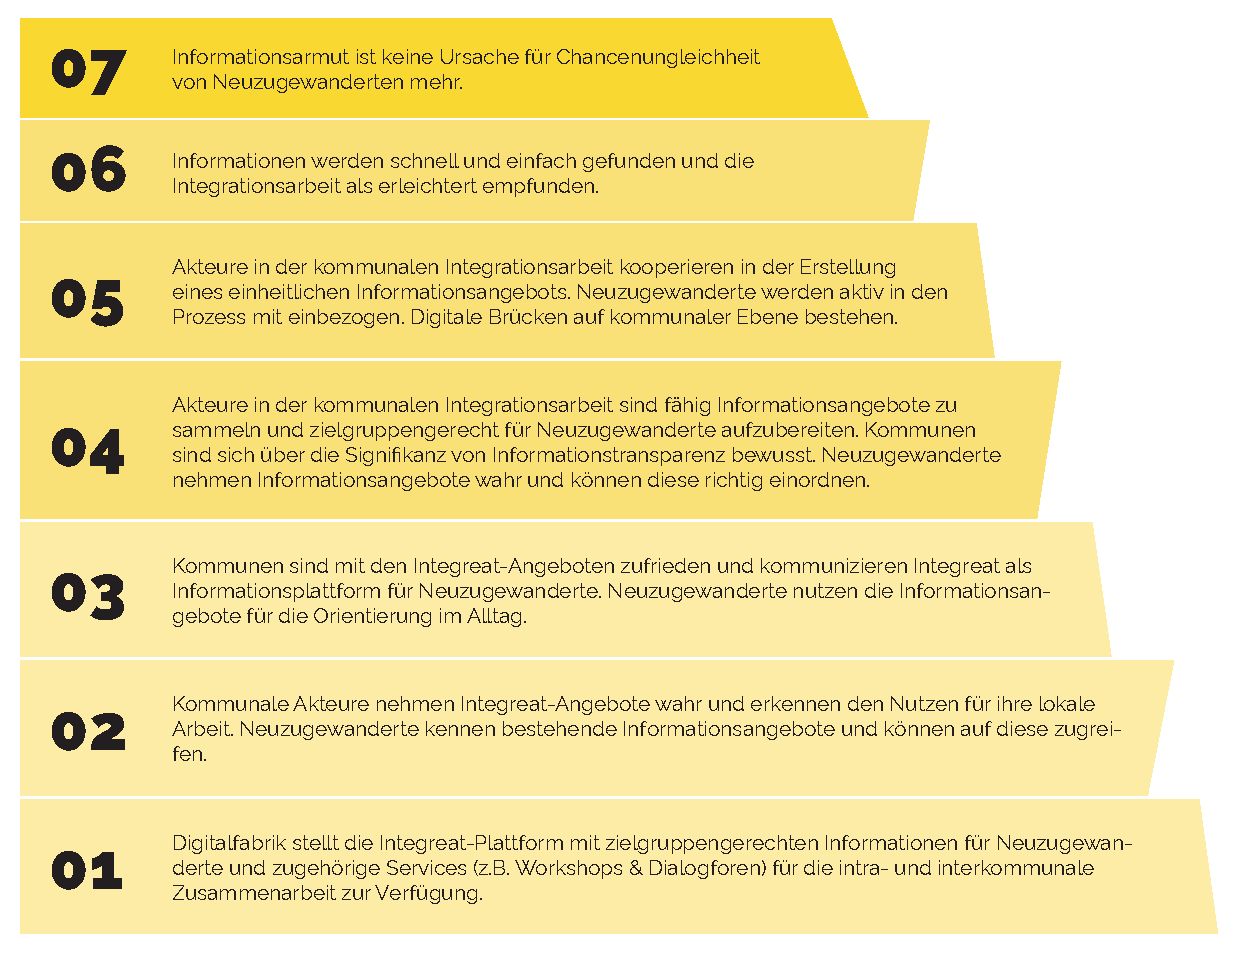
\includegraphics[width=\textwidth,trim=1cm 0.4cm 0.4cm 0.2cm]{Treppengrafik.pdf}
\end{minipage}

\hypertarget{neuzugewanderte-unsere-nutzer}{%
\subsection{Neuzugewanderte – Unsere
Nutzer}\label{neuzugewanderte-unsere-nutzer}}

An erster Stelle in der strategischen Entwicklung und der Arbeit in den
einzelnen Projekten der Digitalfabrik stehen die Bedürfnisse der
neuzugewanderten Menschen in Deutschland. Ausdrücklich werden hierbei
Geflüchtete und Menschen mit Migrationshintergrund miteingeschlossen.
Auch wenn die Gründung der Organisation in Reaktion auf die Zuwanderung
2015 mit vielen geflüchteten Menschen folgte, erfahren wir nach wie vor
in der täglichen Arbeit den besonderen Bedarf für digitale
Unterstützungsangebote zur Integration von allen Menschen, die aus dem
Ausland nach Deutschland kommen.

Die Erweiterung beziehungsweise Öffnung der primären Zielgruppe für die
Angebote um Integreat wird besonders deutlich in der Außenkommunikation
für die Integreat-App. Während die Integreat-App zu Beginn als Angebot
für „Asylsuchende“ deklariert wurde, ging die Entwicklung über
„Flüchtlinge“, zu „Geflüchteten“ über „Menschen mit Migrations- und
Fluchthintergrund“ hin zu dem aktuellen Stand der „Neuzugewanderten“.
Eine eindeutige Unterscheidung zwischen Geflüchteten und anderen
Migrantengruppen ist von Grund auf problematisch, – und für die Arbeit
der Digitalfabrik nicht zwingend notwendig – da die Fluchtsituation
oftmals weitere Migrationsbewegungen mit sich bringt. Dementsprechend
gestalten wir unsere Angebote heutzutage offen zur individuellen lokalen
Gestaltung, um den Herausforderungen vor Ort bestmöglich zu entsprechen.
Die Veränderung stellt sich also sichtbar im Namen dar, betrifft
darunterliegend aber vor allem in Inhalte, Sprachangebot und begleitenden Maßnahmen.

\vspace{0.5cm}

\begin{minipage}[t]{\textwidth}
    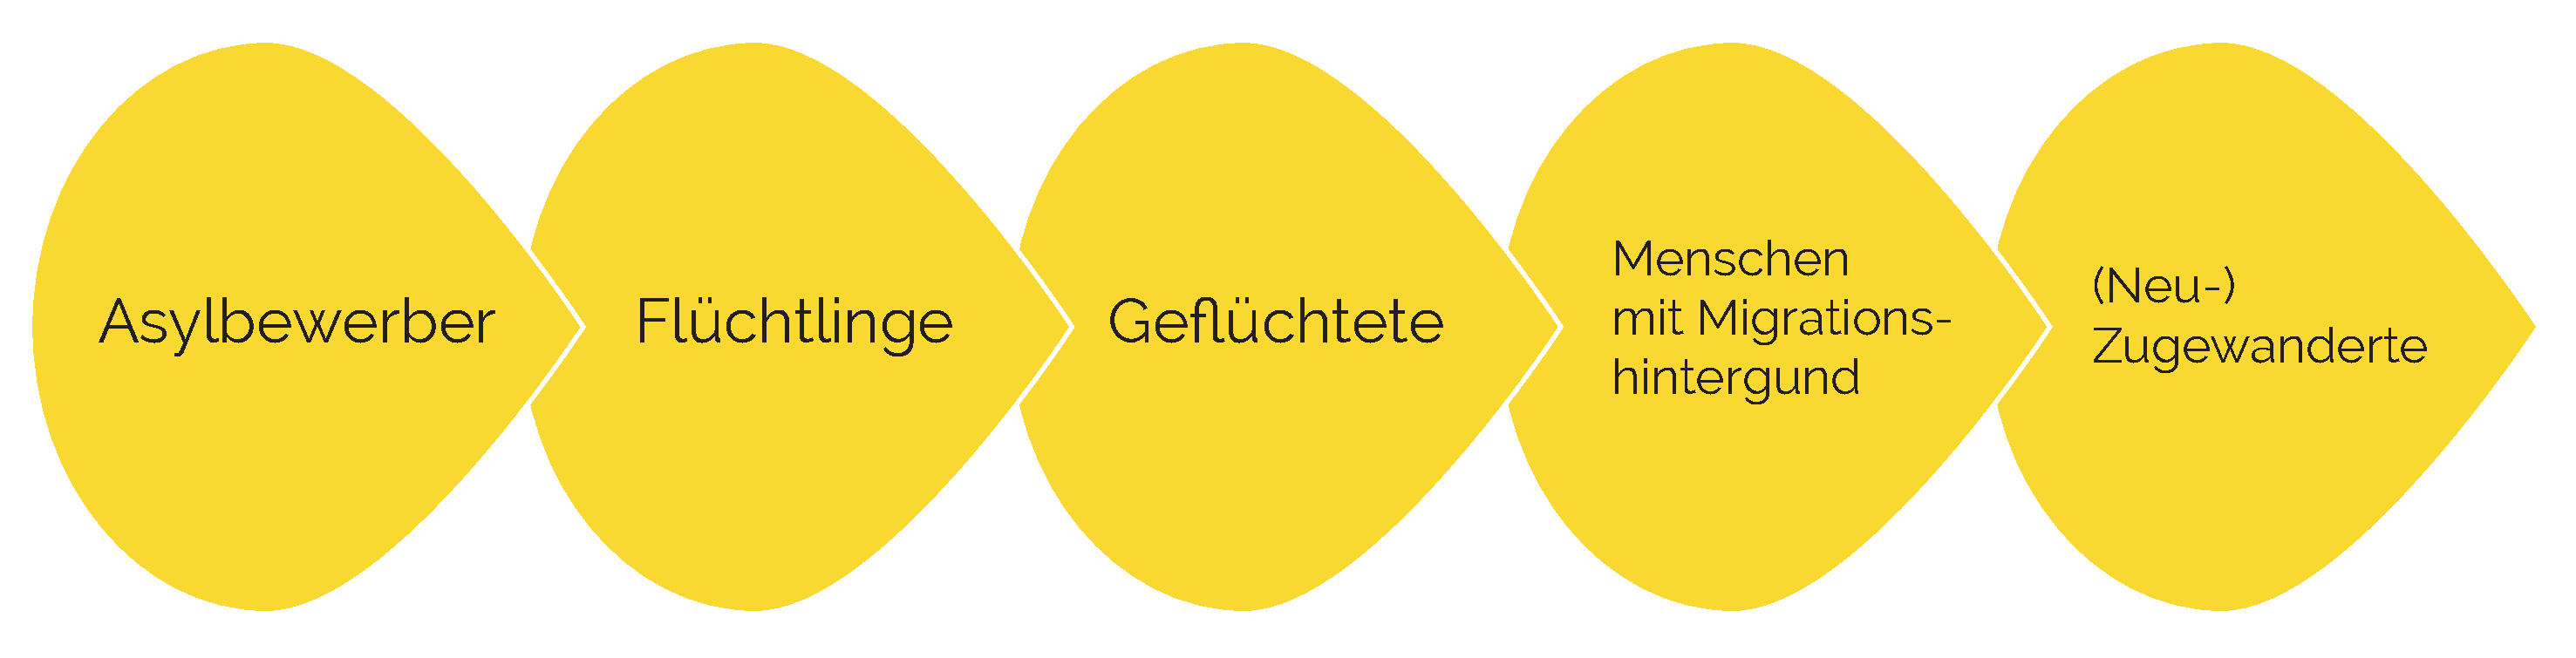
\includegraphics[width=\textwidth]{Flowchart.pdf}
\end{minipage}

\hypertarget{leistungen-output-fuxfcr-neuzugewanderte}{%
\subsubsection{Leistungen (Output) für
Neuzugewanderte}\label{leistungen-output-fuxfcr-neuzugewanderte}}

Unsere Leistungen für die Zielgruppe der Neuzugewanderten im Jahr 2018
beziehen sich in erster Linie auf die App Integreat, deren Betrieb und
technische Weiterentwicklung durch die Digitalfabrik gewährleistet wird.

Anfang des Jahres fand das erste Integreat-Forum mit Geflüchteten und
Neuzugewanderten statt. Dort wurden wichtige aktuelle
Informationsbedarfe evaluiert und redaktionelle Tipps für die kommunalen
Verwalter von Integreat gesammelt. Die Zielgruppe der Neuzugewanderten
möglichst stark in den Weiterentwicklungsprozess von Integreat mit
einzubeziehen ist eine Herausforderung, die auch in den kommenden Jahren
wichtiger Bestandteil unserer Arbeit sein soll. Wir ermutigen
insbesondere auch unsere kommunalen Partner ihre individuelle Zielgruppe
in den Erstellungsprozess und die Evaluation der integreat-App mit
einzubeziehen.

\hypertarget{intendierte-wirkungen-impact}{%
\subsubsection{Intendierte Wirkungen
(Impact)}\label{intendierte-wirkungen-impact}}

Die langfristige Wirkung unserer Aktivitäten für die Zielgruppe der
Neuzugewanderten ist von den kurzfristigen Wirkungen differenziert zu
betrachten, wird jedoch durch diese befördert und in Gang gesetzt.
Kurzfristige Wirkungen werden in der Wirkungslogik als notwendige
Schritte auf dem Weg zu langfristigen Wirkungszielen dargestellt. Bei
dieser langfristigen Wirkung (Impact) lassen sich nur Annahmen darüber
treffen, ob und zu welchem Teil sich diese durch Aktivitäten der
Digitalfabrik entfalten werden. Es besteht an dieser Stelle im Sinne des
wirkungsorientierten Handelns keine Notwendigkeit die messbaren
Entwicklungen einzelnen Akteuren oder Organisationen zuzuordnen und
somit künstliche Konkurrenz zu erschaffen. Soll ein tatsächlicher Wandel
in bestehenden Strukturen entstehen, ist dies eine Aufgabe für Netzwerke
und kann nur im Rahmen von Zusammenarbeit und gemeinsamer
Ressourcennutzung entstehen. Dennoch ist die Benennung der gewünschten
gesamtgesellschaftlichen Wirkung maßgeblich für die strategische
Entwicklung der Organisation und der Zusammenarbeit mit unseren
Partnern. Gemeinsam mit gleichgesinnten Institutionen und Akteuren
können so langfristige Veränderungen bewirkt werden („Smart Networks“).

Durch die Aktivitäten der Digitalfabrik soll die gesellschaftliche
Teilhabe für alle Menschen in Deutschland ermöglicht werden. Teilhabe
bezeichnet die Möglichkeit, Fähigkeit und Verantwortung die Gesellschaft
mitzugestalten in der man lebt. Werden Menschen von der Gesellschaft an
den Rand gedrängt oder gar ausgeschlossen und isoliert, können diese
ihre Bedürfnisse nicht erfüllen und die Möglichkeiten, die ihnen
zustehen würden, nicht nutzen. Eine Gesellschaft, die allen Menschen
Mitbestimmung und Teilhabe ermöglicht, kann allgemeine Ziele unter
Berücksichtigung der verschiedenen Interessengruppen planen und
verwirklichen. Werden bestimmte Personen und Gruppen ausgeschlossen
fehlen wichtige konstituierende Teile.

Das Teilhabeverständnis, das dieser Argumentation zu Grunde liegt,
bezieht sich auf Teilhabe im politischen und kulturellen Leben sowie
allen Formen von Arbeit und der Verfügbarkeit von angemessenem Wohnraum.
Alle genannten Bereiche beeinflussen sich gegenseitig und die
Abhängigkeiten sind komplex. Die Möglichkeit zur Teilhabe im
kulturellen, sozialen, politischen und professionellen Leben ist eine
der wichtigsten Voraussetzungen zur Verwirklichung von
Chancengleichheit. Die Digitalfabrik konzentriert sich vorwiegend auf
die Teilhabe von neuzugewanderten Menschen. Wir sind uns dennoch
bewusst, dass auch andere Interessensgruppen Bedarf an Angeboten zur
Verbesserung der Teilhabe haben und freuen uns Organisationen und
Akteure zu unterstützen, die sich für diese engagieren.

Wichtige Voraussetzung zur gesellschaftlichen Teilhabe von
Neuzugewanderten ist der Abbau von Informationsarmut als Ursache von
Chancenungleichheit in der Gesellschaft. Diese Informationsarmut besteht
insbesondere bei Neuzugewanderten aufgrund von Sprachbarrieren, aber
auch anderem Umgang und anderer Einschätzung von gefundenen
Informationen. Wie aus der Wirkungslogik des Integreat-Projekts deutlich
wird, sind die Voraussetzungen für dieses Ziel u.a. das Informationen
verfügbar sind, gefunden werden, vor allem aber verarbeitet werden
können und die Informationen eine deutliche Verbindung zum Lebensalltag
der Nutzer darstellen. Die Vertrauensbildung in digitale
Informationsangebote zu stärken und zu befördern ist daher ein wichtiges
Anliegen der nächsten Zeit.

\hypertarget{kommunale-verwaltungen-unsere-partner-und-kunden}{%
\subsection{Kommunale Verwaltungen – Unsere Partner und
Kunden}\label{kommunale-verwaltungen-unsere-partner-und-kunden}}

Die Zusammenarbeit mit bereits etablierten und im politischen System
stark verankerten Institutionen wie den kommunalen Verwaltungen
(Kooperation statt Konkurrenz) bietet aufgrund der unterschiedlichen
Kompetenzen für unser soziales Startup ein hohes Synergiepotential und
ist damit die vorrangige Strategie des Unternehmens.

Wir unterscheiden die Zusammenarbeit auf kommunaler Ebene aufgrund der
unterschiedlichen Ansätze in intrakommunale Zusammenarbeit (innerhalb
einer Stadt oder eines Landkreises) und interkommunaler Zusammenarbeit
(im Austausch verschiedener Kommunen und Landkreise untereinander). Die
Leistungen und kurz- bis mittelfristigen Wirkungen unterscheiden sich
einerseits, tragen jedoch im Weiteren zur gleichen Wirkung bei.

\hypertarget{intrakommunale-zusammenarbeit}{%
\subsubsection{Intrakommunale Zusammenarbeit}\label{intrakommunale-zusammenarbeit}}

Zunächst soll im Detail auf die intrakommunale Zusammenarbeit
eingegangen werden. Innerhalb der Kommune beschäftigen sich verschiedene
Institutionen und Stellen mit der Integration Neuzugewanderter. In der
Kommunikation und Zusammenarbeit dieser verschiedenen Akteure besteht
großes Potential für umfassende und erfolgreiche Integrationsarbeit,
dennoch sind aktuell kaum Anknüpfungspunkte vorhanden. Eine neutrale
Plattform zur Kollaboration und regelmäßige Vernetzungstreffen bestehen
häufig nicht. In der Zusammenarbeit der Digitalfabrik als neuem, jungen
Akteur und etablierten Akteuren in Stadt oder Landkreis können alle
voneinander profitieren. Die Digitalfabrik beherrscht digitale
Technologien und kann diese Niederschwellig zur Verfügung stellen,
während die Integrationsakteure vor Ort Erfahrung und Expertise aus der
lokalen Integrationsarbeit in die gemeinsame Arbeit einbringen.

Gleichzeitig existieren auf lokaler Ebene diverse Angebote, Projekte und
Anknüpfungspunkte für neuzugewanderte Menschen. Diese zentral zu sammeln
und übersichtlich darzustellen ist eine wichtige Aufgabe, die nicht nur
direkt den Neuzugewanderten zugutekommt, sondern den
Integrationsakteuren gleichzeitig verdeutlicht, welche Angebote
vorhanden sind und an welchen Stellen möglicherweise noch Lücken
bestehen (Transparenz). Bestehen Inkonsistenzen in den
Informationsangeboten unterschiedlicher Stellen oder fehlen wichtige
Angebote für Neuzugewanderte, wird dies häufig in der Erstellung der
Integreat-Inhalte deutlich und kann behoben werden. Zudem werden alle
Informationen aus dem Integrationsbereich mit der Übertragung in
Integreat auch mehrsprachig nutzbar und können in verschiedenen
Szenarien genutzt werden. Eine neutrale Plattform und einen Anlass zum
Austausch zu bieten sind wichtige Voraussetzungen, um langfristig die
Zusammenarbeit vor Ort zu stärken und somit Integrationsarbeit
wirkungsvoll zu gestalten (Grundlage für digitales Serviceökosystem zur
Integration).

Mit dem Einsatz der Integreat-App und der Zusammenarbeit mit der
Digitalfabrik zeigen kommunale Integrationsakteure große Bereitschaft
zur digitalen Innovation. Sie dienen somit als Leuchtturm und Motivator
für weitere digitale Projekte in der Region. Die Wirkung der
Digitalfabrik entfaltet sich im intrakommunalen Kontext auf die gesamte
Verwaltungsstruktur.

\hypertarget{interkommunale-zusammenarbeit}{%
\subsubsection{Interkommunale
Zusammenarbeit}\label{interkommunale-zusammenarbeit}}

Nicht nur die intrakommunale Komponente stellt in der Arbeit mit den
kommunalen Partnern der Digitalfabrik eine wichtige Komponente dar. Auch
die Vernetzung der einzelnen Kommunen untereinander bietet ein
entsprechendes Potential, um die langfristige Wirkung zu befördern.
Trotz des lokalen Charakters stellt insbesondere die App Integreat ein
wichtiges Verbindungsglied zwischen den verschiedenen aktiven Kommunen
deutschlandweit dar. Durch die Arbeit an einer bundesweiten Plattform,
die dennoch die lokalen Unterschiede abbildet, werden Know-how und
Erfahrungen ausgetauscht und Ressourcen gemeinsam genutzt.

In der interkommunalen Zusammenarbeit, die sich für die Partner der
Integreat-App konkret in der gemeinsamen Nutzung von Inhalten,
Übersetzungen und Technologie äußert, erleben die beteiligten Stellen in
der Kommune direkte Vorteile von Creative Commons und Open Source als
kollaborative Ansätze. Wird ein Inhalt von einer Kommune in Integreat
eingepflegt, kann dieser aufgrund der Creative Commons Lizenz von jeder
anderen beteiligten Kommune genutzt werden. So wird Wissen
weitergegeben, Ressourcen in der Erstellung von Inhalten können geteilt
werden und durch den gemeinsamen Übersetzungsspeicher können sogar
Kosten für Übersetzungen gespart werden.

Alle Entwickelungen der Integreat-Technologie erfolgen quelloffen (Open
Source). Gemeinsam finanzieren alle beteiligten Kommunen neue
Entwicklungen und sorgen für ein nachhaltiges Projekt. Die Open Source
Lizenz ermöglicht es zudem unabhängigen Entwicklern die Lösung zu
überprüfen, andere Projekte können auf die Technologie aufbauen und
Kommunen und Landkreise haben die Möglichkeit Integreat eigenständig auf
ihren Servern aufzusetzen, wenn keine Kooperation mit der Digitalfabrik
erwünscht ist. Durch diese technologische Transparenz entsteht großer
Mehrwert für alle Städte und Landkreise, denn es besteht kein
finanzielles Risiko und Kommunen können mit einem mittleren
vierstelligen Jahresbeitrag am Projekt partizipieren.

Der erlebbare Erfolg schafft Vertrauen in offene Software und geteilte
Inhalte. Gleichzeitig wird das deutschlandweite Netzwerk durch die
Kollaboration gestärkt. So können langfristige Veränderungen in der
gesellschaftlichen Wahrnehmung und Nutzung von Lizenz- und Besitzrechten
erreicht werden.

\hypertarget{leistungen-und-intendierte-wirkungen}{%
\subsubsection{Leistungen und intendierte
Wirkungen}\label{leistungen-und-intendierte-wirkungen}}

Für die Zielgruppe der Kommunen tritt die Digitalfabrik in erster Linie
als Innovationsratgeber auf. Digitalisierung in der kommunalen
Verwaltung und insbesondere in der Integrationsarbeit ist eine komplexe
Herausforderung, der sich kaum junge Unternehmen mit technischem Wissen
annehmen. Das starre und bürokratische Image des öffentlichen Sektors
schreckt viele Startups ab. Dennoch sind die Möglichkeiten der digitalen
Innovation hier besonders groß, denn der Druck den die Digitalisierung
durch das geänderte Nutzerverhalten und die Erwartungen der Bürger an
Angebote ausübt macht keinen Halt vor behördlichen Angeboten.

Mit dem Anspruch von Neutralität berät die Digitalfabrik Kommunen zur
Umsetzung technischer Lösungen, vernetzt und vermittelt. Durch die
Umsetzung von Softwarelösungen sollen Prozesse und Netzwerke unterstützt
und Brücken innerhalb der Gesellschaft geschlagen werden. Workshops vor
Ort tragen zusätzlich zur Vernetzung bei und dienen der
zielgruppengerechten Heranführung an die Technologie. Regionalworkshops
in ähnlichem Format wurden vom Netzwerk IQ bereits für die Vernetzung
kommunaler Akteure als Good Practice ausgezeichnet (http://
www.netzwerk-iq-sachsen.de/dok/GP\_Regionalworkshop\_web.pdf).

Durch den Erfolg der analogen Workshop-Formate wurde das dazugehörige
Workshop-Konzept der Digitalfabrik im Jahr 2018 weiter ausgebaut werden,
um nicht nur Technologien und Prozesse aktiv zu unterstützen, sondern
die Menschen vor Ort stärker in den Gesamtkontext einzubeziehen. So
wurde beispielsweise die Wirkung vor Ort in ausgewählten Kommunen
genauer betrachtet und gemeinsam an Marketingmaßnahmen gearbeitet. In
der Zusammenarbeit mit der bundesweit agierenden Digitalfabrik erkennen
kommunale Akteure Synergiepotentiale und lernen gemeinsam voneinander.

Nach dem großen Erfolg des ersten Integreat-Dialogforums mit Kommunen
und Landkreisen aus ganz Deutschland wurde 2018 ein weiteres Dialogforum
angeboten. Die Teilnahme von fast 50\% unserer Partnerkommunen ist
beispielhaft für den Bedarf an interkommunalem Austausch und wir werden
dieses Angebot in den kommenden Jahren weiter verbessern und ausbauen.

\hypertarget{leistungen-und-wirkungen-aus-weiteren-projekten}{%
\subsubsection{Leistungen und Wirkungen aus weiteren
Projekten}\label{leistungen-und-wirkungen-aus-weiteren-projekten}}

Neben der Weiterentwicklung und dem Betrieb der Integreat-App wurde 2018
insbesondere durch das lokale WLAN-Projekt in Augsburg Wirkung für die
Zielgruppe der Neuzugewanderten generiert.

Die bereits in 2017 mit ganzheitlichem Internetzugang ausgestatteten
Flüchtlingsunterkünfte wurden in 2018 weiter betreut. Eine weitere
Unterkunft kam 2018 hinzu und eine vierte ist für das kommende Jahr in
Planung.

Das von uns betriebene WLAN-Netzwerk kann von den Bewohnern der
Unterkunft für 5 Euro im Monat genutzt werden. Häufig besteht keine
(stabile) Internetverbindung in den Aufnahmeeinrichtungen für
geflüchtete Menschen. Diese ist jedoch essentiell, um den Kontakt mit
der Heimat und der Familie aufrecht zu halten sowie Informationen zu
Rechten und Möglichkeiten in Deutschland (bspw. Ausbildungsmöglichkeiten
oder Asylrecht) selbstständig und selbstverantwortlich akquirieren zu
können. Der Ausbau von Internetzugang in weiteren
Flüchtlingsunterkünften in der Umgebung wurde evaluiert.

Diese Leistungen zeigen unmittelbare Wirkungen bei der Zielgruppe. Sie
haben einen direkten Einfluss auf die Zugänglichkeit und Transparenz von
Informationen, in diesem Fall in Form von Online-Informationsangeboten.
Gleichzeitig wird die Eigenständigkeit der Neuzugewanderten gestärkt, da
diese befähigt werden sich unabhängig von Personen und Institutionen vor
Ort selbstverantwortlich einen Überblick zu verschaffen. Zudem können
Informationen, die über einen digitalen Weg gewonnen wurden im Alltag
eingesetzt werden und als Brückenfunktion zu realen persönlichen
Kontakten führen. Eine Brückenfunktion stellen digitale Angebote dar,
denen es gelingt einen konkreten Einfluss auf die Lebenswirklichkeit der
Nutzer auszuüben. Beispielsweise wird eine online gefundene
Beratungsstelle tatsächlich aufgesucht und ein Beratungsgespräch kommt
zustande. Dieser Realitätsbezug ist für die Wirkung digitaler Angebote
zur Integration besonders wichtig, da sie die Lebenswirklichkeit der
Nutzer tatsächlich beeinflusst.

\hypertarget{ressourcen-leistungen-und-wirkung-im-berichtzeitraum-eine-aufstellung}{%
\section{Ressourcen, Leistungen und Wirkung im Berichtzeitraum – Eine
Aufstellung}\label{ressourcen-leistungen-und-wirkung-im-berichtzeitraum-eine-aufstellung}}

\hypertarget{eingesetzte-ressourcen-input}{%
\subsection{Eingesetzte Ressourcen (Input)
}\label{eingesetzte-ressourcen-input}}

Die finanziellen Ressourcen setzen sich im Jahr 2018 aus Personalkosten
in Höhe von 89.000 Euro und Sachkosten in Höhe von 35.000 Euro zusammen.
Insgesamt wurden im Jahr 2018 somit 124.000 Euro zur Weiterentwicklung
der Organisation und der Verbesserung der Integrationsarbeit
deutschlandweit eingesetzt.

Mit einer fluktuierenden Zahl von circa 20 sehr engagierten
Ehrenamtlichen kommen zeitliche Ressourcen von geschätzten 5.000 Stunden
hinzu. Ein großer Teil der ehrenamtlichen Arbeit trug zur technischen
Weiterentwicklung der Integreat-App bei. Der Großteil der hauptamtlichen
Beschäftigten speist sich aus vormals ehrenamtlich Engagierten.

\hypertarget{erbrachte-leistungen-und-wirkungen}{%
\subsection{Erbrachte Leistungen und
Wirkungen}\label{erbrachte-leistungen-und-wirkungen}}

Aufbauend auf den Leistungen und Wirkungen des letzten Jahres konnte die
Digitalfabrik im Jahr 2018 weitere Fortschritte für die primäre
Zielgruppe der Neuzugewanderten sowie auf kommunaler Ebene erzielen.
Ende 2018 steht die Integreat-App in 48 Städten und Landkreisen in
Deutschland zur Verfügung und hilft dort die Informationsvermittlung an
Neuzugewanderte erfolgreich mitzugestalten. Die Steigerung der
Integreat-Kommunen wirkt sich einerseits auf die Zielgruppe der
Neuzugewanderten aus, da ein größerer Anteil dieser durch Integreat mit
lokalen Informationen versorgt werden kann. Andererseits profitieren
auch die kommunalen Partner der Digitalfabrik im interkommunalen Bereich
von einer wachsenden Community, da mehr Inhalte und Übersetzungen
produziert werden, die wiederum gemeinschaftlich genutzt werden können
und zu Kosten- und Zeitersparnissen führen.

2018 wurde der Bereich Wohnen durch die Entwicklung einer Wohnraumbörse
ausgeweitet. Rückblickend konnte die Wohnraumbörse ihre Wirkung nicht
entfalten. Die schwierige Situation für Neuzugewanderte im Bereich
Wohnungssuche konnten aufgrund der diversen Einflussfaktoren nicht in
dem Umfang durch unsere digitale Lösung verbessert werden wie
ursprünglich erwartet. Trotz der jährlichen Fokussierung auf einen
Teilbereich der Integration wird in der strategischen Entwicklung der
Digitalfabrik stets die Interdependenz der einzelnen Bereiche bedacht
und nach Möglichkeit Angebote in allen vier Teilbereichen geschaffen.

Durch die Aktivitäten der Digitalfabrik konnten nachweislich im Jahr
2018 vor allem Wirkungen auf kommunaler Ebene und im interkommunalen
Austausch erreicht. Als Indikatoren für diese Wirkungen dienen vor allem
persönliche Berichte und Feedback aus den Kommunen bzw. vom
Integreat-Dialogforum in Nürnberg im November 2018 sowie Beobachtungen
der Mitarbeitenden inder Digitalfabrik.

Auch in 2018 konnte eine hohe Bereitschaft beobachtet werden, an
Integreat Workshops und Veranstaltungen sowie dem Integreat-Dialogforum
teilzunehmen. Diese Teilnahmebereitschaft zeigt den großen Bedarf und
den wichtigen Beitrag, den die Veranstaltungen zur Arbeitsfähigkeit und
dem Erfolg der Integrationsarbeit leisten, da die Veranstaltungen
zeitintensiv sind und die Bereitschaft zur Teilnahme von verschiedenen
Integrationsakteuren lässt vermuten, dass ein Mehrwert für die
Teilnehmer erkennbar ist.

Zudem wurden bereits 7 Kooperationsvereinbarungen nach der Laufzeit von
zwei Jahren verlängert. Dies ist ein Indikator dafür, dass ein
signifikanter Mehrwert in der Integrationsarbeit vor Ort durch den
Einsatz der Integreat-App und die inter- sowie intrakommunale
Vernetzung, die durch Integreat vorangetrieben wird, besteht.

\hypertarget{mauxdfnahmen-zur-begleitenden-evaluation-und-qualituxe4tssicherung}{%
\subsection{Maßnahmen zur begleitenden Evaluation und
Qualitätssicherung}\label{mauxdfnahmen-zur-begleitenden-evaluation-und-qualituxe4tssicherung}}

\hypertarget{integreat-dialogforen}{%
\subsubsection{Integreat-Dialogforen}\label{integreat-dialogforen}}

Nachdem im November 2017 das erste Integreat-Dialogforum an der
Technischen Universität in München stattfand, gab es eine erfolgreiche
Wiederholung dieses interkommunalen Austauschs im November 2018. Im
Nürnberger Rathaus kamen 32 Personen aus 22 unterschiedlichen Kommunen
zusammen, um sich sowohl im Plenum als auch in kleineren Workshops über
relevante Themen bezüglich der App auszutauschen. Dem Dialog wurde ein
Input seitens des Integreat-Teams vorangestellt, der zu Beginn noch
einmal verdeutlichen sollte, wie wir auf die Zusammenarbeit von App und
Kommunen blicken und welche Vorteile die Vernetzungstätigkeit von
Integreat auch für die Kommunen untereinander bereithält. Hier wurde
verdeutlicht, wie wichtig die Mitarbeit der kommunalen Partner für das
gemeinsame Vorankommen ist. Voneinander zu lernen und sich gegenseitig
zu unterstützen ist ausschlaggebend, um langfristig und erfolgreich die
Integration von neuzugewanderten Menschen in den verschiedenen Regionen
zu verbessern. Die anschließende Plenumsdiskussion wurde neben Problemen
und Möglichkeiten der Zielgruppenerreichung vom Thema Sprache dominiert.
Genauer waren der Einsatz von einfacher Sprache und generell das Thema
Barrierefreiheit, sowie Aktualisierung und Übersetzungen von
Integreat-Inhalten Teil der Diskussion. Darüber hinaus fanden in zwei
parallelen Workshops folgende Themen Eingang in die Diskussion: „Reden
wir über Inhalte“ und „Reden wir über 2021“. Hier wurde seitens der
Kommunen vor allem die Niedrigschwelligkeit der App gelobt und für die
zukünftige Arbeit weiterhin als relevant herausgestellt.

Der angeregte Austausch des Dialogforums brachte nicht nur neuen Input
für die Kommunen mit sich (wie aus der Evaluation der Veranstaltung
hervorgegangen ist), sondern hilft auch der Digitalfabrik dabei
weiterhin nah an den Partnern zu bleiben. Damit wird gewährleistet, dass
auf Veränderungen seitens der Kommunen eingegangen werden kann und die
Qualität des Angebots stabil bleibt. Durch das Dialogforum konnte
qualitativ herausgestellt werden, wie die einzelnen Partner arbeiten und
in welchem Teil des Prozesses mit der App sie Unterstützung von der
Digitalfabrik benötigen. Vor allem in Hinblick auf die Kosten von
Integreat (Betrieb und Übersetzungen) wünschen sich die Kommunen mehr
Unterstützung. Aufgrund des durchweg positiven Feedbacks zu diesem Event
wird auch im kommenden Jahr ein Dialogforum stattfinden.

\hypertarget{wissenschaftliche-evaluationen}{%
\subsubsection{Wissenschaftliche
Evaluationen}\label{wissenschaftliche-evaluationen}}

Ein Aspekt auf den seit der Gründung 2016 viel Wert gelegt wurde ist die
wissenschaftliche Evaluierung der Integreat-App. Im Jahr 2018 wurden
zahlreiche Arbeiten verfasst, die sich mit der Bedeutung von
Informations- und Kommunikationstechnik (ICT) im Kontext der Integration
auseinandersetzen.

Daniel Kehne legte mit seiner Masterarbeit an der TU München dar, dass
digitale Technologien für Geflüchtete ein entscheidendes Instrument für
die Teilhabe an der Gesellschaft sind. Aus Interviews mit Menschen mit
Fluchthintergrund konnte mit Hilfe einer qualitativen Analyse abgeleitet
werden, dass die Nutzung von ICTs einen indirekten Einfluss auf die
Teilhabe haben, da durch Informationsplattformen – wie Integreat –
wichtige Aspekte an Neuzugewanderte weitergegeben werden können.

Ebenfalls zu digitalen Technologien als Kommunikationsmittel von
Geflüchteten forschte Hannah Diemer an der Universität Augsburg im
Rahmen ihrer Abschlussarbeit. Die Nutzung von ICTs unterstützt durch die
Weitergabe von Informationen bei der Ankunft in Deutschland. Durch das
Netzwerk, welches sich über soziale Medien aufbauen lässt, fällt es
leichter sich in eine Gesellschaft einzufinden und Freunde oder Bekannte
zu finden und damit das eigene soziale Kapital zu erweitern. Dies
vereinfacht letztendlich ebenfalls den Integrationsprozess. Damit wurde
verdeutlicht, dass im Zeitalter der Digitalisierung und mit dem Internet
die Integration durch die besseren Möglichkeiten zur Kontaktaufnahme
vereinfacht wird. Als Fazit für die Arbeit der Digitalfabrik kann aus
der genannten Forschungsarbeiten gezogen werden, dass durch unser
Auftreten auf dem digitalen Feld ein deutlicher Mehrwert für die
Zielgruppe erreicht werden kann und die Nutzung von Informationen aus
der Integreat-App auf dem Weg in die Gesellschaft eine Hilfestellung
ist.

Einen besonderen Stellenwert im Hinblick auf die wissenschaftliche
Evaluation nimmt zudem die Bachelorarbeit von Janine Rosenbaum an der TU
München ein, die als Case History in Zusammenarbeit mit Robert Zepic,
Clara Bracklo, Maximilian Schreieck, Dr. Manuel Wiesche und Prof. Dr.
Helmut Krcmar den Digital Government Excellence Award 2018 auf der 18.
European Conference on Digital Government (ECDG) in Spanien gewann. Die
Forschungsarbeit trägt den Titel “Integreat: An information ecosystem
for refugees“. Die Arbeit zeigt auf welche Gründe es für die
Nicht-Nutzung von Mobile Government gibt. Das Resultat ist, dass nicht
das Angebot selbst verantwortlich dafür ist, wenn es nicht genutzt wird,
sondern hier eher Sprachbarrieren oder die Unbekanntheit des Angebots
wirken. Daraus ziehen wir die Notwendigkeit Integreat durch Verbesserung
der Marketing-Maßnahmen noch weiter zu verbreiten und bekannt zu machen,
um den negativen Auswirkungen einer digitalen Kluft entgegen zu wirken.

Die Masterarbeit an der Pädagogischen Hochschule Schwäbisch Gmünd von
Georg Meyer erarbeitete Inhalte, die Neuzugewanderte aus einer
bestimmten Kommune brauchen, um diese schlussendlich in die
Integreat-App einzupflegen. Hieraus lassen sich Bedarfe ableiten, die
auf die benötigten Inhalte für eine erfolgreiche Integration hinweisen.
Die Relevanz der wissenschaftlichen Arbeiten, die im Kontext von
Integreat bereits verfasst wurden, ist enorm. Daher werden
Forschungsarbeiten, die das Wirken der Digitalfabrik thematisieren auch
zukünftig einen wichtigen Bestandteil der Unternehmensstrategie bilden.

\hypertarget{planung-und-ausblick}{%
\section{Planung und Ausblick}\label{planung-und-ausblick}}

\hypertarget{planung-und-ziele}{%
\subsection{Planung und Ziele}\label{planung-und-ziele}}

Unsere Organisation nimmt Fahrt auf. Das vor allem in der Planung des
neuen Jahres deutlich. Durch personelle Erweiterungen in der
Digitalfabrik soll diese Entwicklung in die richtige Richtung gelenkt
werden. Die vier großen Ziele sind:

\begin{enumerate}
\def\labelenumi{\arabic{enumi}.}
\item
\textbf{Professionalisierung und Ausweitung der Kooperation mit
unseren kommunalen Partnern}

Bereits unter Punkt 3.3 geht hervor, dass die inter- und intrakommunale
Zusammenarbeit für unsere Wirkung essentiell ist. Zudem wächst die
Anzahl der Integreat-Kommunen beinahe monatlich an und somit steigt
nicht nur das Potential der Zusammenarbeit, sondern auch der
Betreuungsaufwand auf unserer Seite an. Wir haben uns dafür entscheiden
den Wind dieser Entwicklung zu nutzen und haben eine neue Stelle zur
Betreuung der Kommunen und Landkreise geschaffen. So können wir
langfristig die enge Zusammenarbeit garantieren.

Eine weitere Entwicklung die bereits beobachten und stark unterstützen
ist die Zusammenarbeit zwischen mehreren Integreat-Kommunen auf
inhaltlicher Ebene. Besonders naheliegend ist die Zusammenarbeit von
Landkreis und Stadt, aber auch andere Kooperationen in Form von
inhaltlichem Austausch sind sehr ertragreich. 2019 sollen solche
Potentiale weiter ausgelotet werden und möglicherweise sogar größere
Regionen zur kooperativen Umsetzung von Integreat ermutigt werden.

\item
\textbf{Fokus Arbeitsmigration}

Arbeitsmarktbezogene Zuwanderung stellt eine große Chance für unsere
Gesellschaft und für die betroffenen Menschen dar. Die Zahl der
Erwerbstätigen in Deutschland wird abnehmen und das Interesse an
gesteigerter Arbeitsmigration bringt für viele Städte und Landkreise die
Notwendigkeit mit sich, für qualifizierte Menschen im Ausland offen und
attraktiv zu zeigen. Aktuell wird dieser Gesichtspunkt nur indirekt
durch den Einsatz von Integreat bedient. In Zukunft soll es Kommunen und
Landkreisen durch gezielt arbeitsmarktspezifische Inhalte noch besser
möglich sein, Arbeitsmigration zu fördern und gleichzeitig die
ankommenden Menschen durch hohe Informationstransparenz gut
einzubeziehen. Menschen, die gezielt nach Deutschland kommen, um hier
eine Arbeitsstelle anzutreten, haben sie wenig Zeit persönliche
Beratungsdienste in Anspruch zu nehmen. Daher ist es entscheidend, dass
Informationen zu Alltag und Gesellschaft digital und gesammelt verfügbar
sind. Denn auch für Arbeitsmigrantinnen und Arbeitsmigranten sind
ganzheitliche lokale Informationen zu allen Lebensbereichen wichtig, um
sich in der Gesellschaft einleben zu können und in ihrem neuen Wohnort
Fuß zu fassen.

\item
\textbf{Integreat Europe}

Das Konzept hinter Integreat – Informationen lokalspezifisch und
mehrsprachig über App und Website zu verbreiten – bedient ein
Problemfeld, das nicht nur im deutschen Raum akut ist, sondern auch
viele andere Länder betrifft. Informationen sind in der modernen
Informationsgesellschaft leider noch nicht so zugänglich wie es auf den
ersten Blick wirkt und Disparitäten im Informationszugang erschweren
vielen Menschen das Leben. Integreat ist ein einfach umzusetzendes und
niederschwelliges Angebot, das Organisationen oder Verwaltungen zur
Verbesserung dieser Situation nutzen können.

In 2019 sollen die Grundlagen geschaffen werden, um Integreat auch
außerhalb der Landesgrenzen sichtbar und nutzbar zu machen.

\item
\textbf{Denkfabrik als Innovationsinkubator}

Die Digitalfabrik existiert seit 2016 und hat sich in den letzten Jahren
vor allem mit dem Projekt Integreat etabliert und Wirkung erzielt. In
dieser Zeit hat das Team viele Erfahrungen zur erfolgreichen
Projektarbeit gesammelt und gleichzeitig wurde der Bedarf an weiteren
Initiativen, die digitale Technologien mit aktuellen Bedarfen in der
sozialen und öffentlichen Arbeit kombinieren, deutlich.

In 2019 wird mit der Schaffung von neuen Stellen genau dieses Potential
genauer beleuchtet. Entstehen sollen daraus Projekte hohes
Transferpotential, leichte Zugänglichkeit für die Nutzer und
selbstverständlich in besonderem Maße zur Verbesserung der
Lebenssituation von Menschen beitragen, die unter den aktuellen
Umständen in der Gesellschaft benachteiligt sind.

In der Beschreibung unserer Ziele für das kommende Jahr wird deutlich,
dass wir uns nicht auf unserem Erfolg der letzten Jahre ausruhen,
sondern nach immer neuen Herausforderungen suchen. Wir sind
entschlossen, die Erfahrungen aus dem Integreat-Projekt zu nutzen, um
weitere Projekte umzusetzen, deren Notwendigkeit uns aus unserer
täglichen Arbeit immer wieder bewusst wird.

\end{enumerate}

\hypertarget{chancen-und-risiken}{%
\subsection{Chancen und Risiken}\label{chancen-und-risiken}}

Wie bereits in den unterschiedlichen Zielsetzungen deutlich geworden
ist, bestehen für die Digitalfabrik und das Projekt Integreat im
kommenden Jahr viele Potentiale zur Weiterentwicklung. Der Bedarf am
Integreat-Projekt ist nach wie vor gegeben. Wie bereits im letzten
Wirkungsbericht vorhergesehen hat sich in der kommunalen
Integrationsarbeit eine Bewegung in der Zielgruppe von Integreat
vollzogen und Integration wird vermehrt im Kontext von EU-Migration
betrachtet. Integration von Geflüchteten steht nicht mehr im gleichen
Umfang im Mittelpunkt der Aufmerksamkeit wie noch vor einigen Jahren und
in diesem Sinne sind Fördergelder weniger verfügbar. Die
Finanzierbarkeit von Projekten wie Integreat wird dadurch nicht nur für
uns als Organisation, sondern auch für unsere Partnerkommunen
herausfordernder. Die auf dem Dialogforum im November 2018 diskutierten
Punkte sollen u.a. in ein faireres Preismodell und einen neuen Ansatz
zur Entlastung bei den Übersetzungskosten überführt werden. Wie bereits
in den vergangenen Jahren versuchen wir Veränderungen bei unseren Kunden
und Nutzern vorausblickend entgegenzuwirken, indem wir unsere Projekte
flexibel aufbauen und zudem weitere digitale Projekte zu anderen
gesellschaftlichen Problematiken in Betracht ziehen.

Neben den gesellschaftlichen Entwicklungen, die die Arbeit der
Digitalfabrik beeinflussen, sehen wir auch internen Veränderungen in
unserer Organisation, die gleichzeitig große Chancen und Risiken mit
sich bringen. Die Digitalfabrik professionalisiert sich zunehmend und
einige ehemals ehrenamtlichen Mitarbeitende wurden hauptamtlich
angestellt. Gleichzeitig bestehen zwischen Hauptamtlichen und
Ehrenamtlichen teilweise große Unterschiede in dem Umfang ihrer Arbeit
für das Integreat-Projekt. Um zu vermeiden, dass Ehrenamtliche abgehängt
werden und ihren Beitrag zum Projekt nicht mehr leisten können, sind die
bezahlten Wochenstunden intern auf 20 Stunden pro Projekt gedeckelt.

\hypertarget{organisationsstruktur-und-team}{%
\section{Organisationsstruktur und
Team}\label{organisationsstruktur-und-team}}

\hypertarget{organisationsstruktur}{%
\subsection{Organisationsstruktur}\label{organisationsstruktur}}

Das circa 29-köpfige Team setzt sich zum größten Teil aus Ehrenamtlichen
zusammen. Zusätzlich kann die Digitalfabrik auf die Arbeit von sieben
hauptamtlichen Mitarbeitern sowie im Jahr 2018 auf 2 Honorarkräfte
zurückgreifen. Der Gedanke des „Community Engagement” , bei dem wenige
Hauptamtliche eine große Anzahl Ehrenamtlicher koordinieren, ist
weiterhin ersichtlich, durch die zunehmende Übernahme von Ehrenamtlichen
ins Hauptamt und stärkere Professionalisierung jedoch etwas verflacht.
Die verschiedenen Arbeitsbereiche werden je nach Bedarf von größeren
oder kleineren Teams abgedeckt. Ein großer Teil der Mitarbeitenden
absolviert parallel ein Studium, sodass unsere Organisation auf
individuelle Arbeitszeitmodelle und dynamische Anforderungen an die
Projektkoordination reagieren können muss. Personen, die schon länger
Teil des Teams und Projekts sind, dienen intern als Berater und kümmern
sich um das Einarbeiten von neuen Mitarbeitern. Hauptamtliche
Mitarbeiter stehen in den einzelnen Arbeitsbereichen als Kontante und
Ansprechpartner für Unklarheiten und operative Herausforderungen mit
zeitlichen Fristen zur Verfügung. Auf den vierteljährlich stattfindenden
Integreat-Konferenzen der Digitalfabrik treffen sich alle Mitarbeiter
physisch für zwei Tage und können sich über aktuelle Aufgaben,
Herausforderungen, Bedarfe und Entwicklungen austauschen sowie gemeinsam
strategische Meilensteine und Ziele definieren. So wird auch in einer
virtuellen Organisation, deren Mitglieder sich über verschiedene Teile
Deutschlands erstrecken, gute Zusammenarbeit und eine gemeinsame
Organisationskultur erhalten.

\hypertarget{kooperationen-partnerschaften-und-netzwerke}{%
\subsection{Kooperationen, Partnerschaften und
Netzwerke}\label{kooperationen-partnerschaften-und-netzwerke}}

Historisch bedingt spielen die Gesellschafter der Digitalfabrik auch im
Bereich der Partnerschaften, Kooperationen und Netzwerke eine zentrale
Rolle. Über den Hauptgesellschafter, den Tür an Tür e.V., besteht eine
starke Vernetzung mit Integrationsprojekten in Augsburg. Der Verein
existiert seit 1992 in Augsburg und setzt sich seitdem in regionalen
Projekten für die Chancen und Rechte von Migrantinnen und Migranten ein.
Die Schwesterunternehmung der Digitalfabrik, die Tür an Tür –
Integrationsprojekte gGmbH, ist die Schnittstelle zum bundesweit
agierenden Netzwerk IQ und dem bayerischen Landesnetzwerk MigraNet, das
dort koordiniert wird. Abgesehen von der finanziellen Förderung des
Netzwerks, die zum 31.12.2018 ausläuft, profitiert die Digitalfabrik vom
gesammelten Know-how aus über 400 Teilprojekten in ganz Deutschland aus
dem Themenbereich der Integration von Migrantinnen und Migranten in den
deutschen Arbeitsmarkt.

Die übrigen Gesellschafter, ihres Zeichens Mitarbeiter der TU München,
bringen nicht nur ihre Expertise im Bereich der Softwarearchitektur ein,
sondern öffnen auch regelmäßig ihre Kontakte in die nationale
E-Government-Szene und zu anderen Forschungseinrichtungen. Darüber
hinaus ist der Lehrstuhl für Wirtschaftsinformatik nach wie vor
Ausrichter der vierteljährlichen Konferenzen des Integreat-Projekts,
Forschungspartner für diverse Problemstellungen der Digitalfabrik und
Betreuer von Abschlussarbeiten im Kontext der Tätigkeiten der
Digitalfabrik. Regelmäßig wird die Digitalfabrik in Lehrveranstaltungen
und Seminaren als Praxispartner einbezogen.

Die im Laufe des Jahres 2017 geschlossenen Partnerschaften mit der
Vereinigung der Bayerischen Wirtschaft e.V. für die Praktikumsbörse
„sprungbrett into work“, und mit der Handwerkskammer für den
„Lehrstellenradar“ bestehen auch weiterhin. Die genannten Plattformen
konnten über Schnittstellen in die Integreat-App integriert werden, ohne
dass Ressourcen für neue Entwicklungen von der Digitalfabrik aufgewendet
werden mussten. Die Kooperationen steigern die Wirkung auf allen Seiten.

Die Partnerschaft mit dem Übersetzungsbüro tolingo zeigte im
zurückliegenden Jahr ihr Potenzial durch eine größere Inanspruchnahme
von Kommunen und Kreisen. Der stark gewachsene „Translation Memory“
verhilft den Kommunen und Kreisen zu deutlichen Einsparungen beim
Einkauf der Übersetzungsdienstleistungen. Als Resultat dieser
erfolgreichen Zusammenarbeit soll der bestehende Rahmenvertrag abgelöst
werden und mit einem breiteren Sprachangebot und weiter verbesserten
Konditionen erneuert werden.

Die Digitalfabrik war ausgewählte Teilnehmerin der „Teilhabe
Wirkungsschmiede“ des „Programm Engagement mit Perspektive“ von Ashoka
Deutschland. Gemeinsam mit anderen Sozialunternehmen wurde insbesondere
die Wirkungsausrichtung der jeweiligen Aktivitäten auf den Prüfstand
gestellt. Die grundlegende Ausrichtung der Strategien der Digitalfabrik
sind von diesem Austausch geprägt. Als Alumni des Programms ist die
Digitalfabrik zudem Teil eines großen Netzwerks von Unternehmungen mit
denselben Werten und Visionen.

Ein wichtiges Ereignis im Jahr 2018 war die Teilnahme und die
Auszeichnung als Leuchtturmprojekt der Google.org Impact Challenge
erhalten. Teil der Auszeichnung ist nicht nur das Preisgeld von 250.000
Euro, sondern auch die mögliche Unterstützung durch eine Google
Mitarbeiterin, die uns unter anderem dabei helfen kann auf bestimmte
Google Ressourcen zuzugreifen. Es besteht zudem ein regelmäßiger
Austausch mit den anderen Leuchtturmprojekten und wir sind überzeugt,
dass somit entstehende Netzwerk durch unsere Erfahrungen bereichern und
gleichzeitig in der Zusammenarbeit neue Synergien entwickeln zu können.

\hypertarget{organisationsprofil}{%
\section{Organisationsprofil}\label{organisationsprofil}}
\hypertarget{allgemeine-angaben}{%
\subsection{Allgemeine Angaben}\label{allgemeine-angaben}}

\begin{adjustwidth}{-1cm}{-1cm}
\begin{tabularx}{\textwidth+2cm}{p{5cm}X}
\toprule
Name & Tür an Tür – Digital Factory gGmbH\tabularnewline
\midrule
Sitz der Organisation gemäß Satzung & Augsburg\tabularnewline
\midrule
Gründung & 22.06.2016\tabularnewline
\midrule
Rechtsform & gemeinnützige GmbH\tabularnewline
\midrule
\begin{minipage}[t]{0.47\columnwidth}\raggedright
Kontaktdaten\strut
\end{minipage} & \begin{minipage}[t]{\columnwidth}
Wertachstr. 29

86153 Augsburg

\href{mailto:digitalfactory@tuerantuer.de}{\url{digitalfactory@tuerantuer.de}}

\url{https://tuerantuer.de/digitalfabrik/}
\end{minipage}\tabularnewline
\midrule
Link zur Satzung (URL) & \url{https://tuerantuer.de/wp-content/uploads/2017/05/Gesellschaftsvertrag\_TATDF\_final.pdf}\tabularnewline
\midrule
Registeramt & Finanzamt Augsburg-Stadt\tabularnewline
Registernummer & HRB30759\tabularnewline
Datum der Eintragung & 27.06.2016\tabularnewline
\midrule
Angabe über die Gemeinnützigkeit gemäß §52 Abgabenordnung. Datum des
Feststellungsbescheids, Ausstellendes Finanzamt, Erklärung des
gemeinnützigen Zwecks & Gemeinnützigkeit gemäß §52 Abgabenordnung
festgestellt am 13.09.2016 vom Finanzamt Augsburg-Stadt (1) Gegenstand
des Unternehmens ist die Anbahnung und Durchführung von Projekten auf
digitaler Basis, die die Integration von Menschen mit Migrations- oder
Fluchthintergrund in die Gesellschaft und in den Arbeitsmarkt fördern
sollen. (2) Der Unternehmensgegenstand wird insbesondere durch folgende
Maßnahmen verwirklicht: a. Durchführung von Projekten, die die
Integration selbst, die Bereitschaft zur Integration, den
interkulturellen Informationsaustausch oder das Zusammenleben von
Menschen mit Flucht- oder Migrationshintergrund unter Einbezug von
digitalen Lösungen verbessern; b. Durchführung von Projekten, die
Beratung, Qualifizierung und Informationsbereitstellung für Menschen mit
Migrations- oder Fluchthintergrund unter Einbezug von digitalen Lösungen
unterstützen; c. Erarbeitung digitaler Lösungen, die die Arbeit und
Organisation im öffentlichen und sozialen Sektor
verbessern.\tabularnewline
\midrule
Anzahl MitarbeiterInnen & 29 \tabularnewline
davon hauptamtlich & 7 \tabularnewline
davon Honorarkräfte & 2 \tabularnewline
davon ehrenamtlich & 20 \tabularnewline
\bottomrule
\end{tabularx}
\end{adjustwidth}

\hypertarget{governance-der-organisation}{%
\subsection{Governance der
Organisation}\label{governance-der-organisation}}

\hypertarget{leitungs--und-geschuxe4ftsfuxfchrungsorgan}{%
\subsubsection{Leitungs- und
Geschäftsführungsorgan}\label{leitungs--und-geschuxe4ftsfuxfchrungsorgan}}

Die Tür an Tür - Digitalfabrik wird von Daniel Kehne und Fritjof Knier
als gleichberechtigte Geschäftsführer nach außen vertreten. Beide
Geschäftsführer sind alleinvertretungsberechtigt und üben diese Aufgabe
ehrenamtlich aus. Daniel Kehne wurde 1990 im westfälischen Ahlen
geboren. Nach dem Abitur auf einem technischen Gymnasium absolvierte er
ein duales Studium in der IT-Sparte der Siemens AG. Ab 2012 arbeitete er
als Prozessberater beim französischen IT-Konzern Atos. Von 2014 bis 2018
studierte er an der Universität Augsburg und TU München Finance \&
Information Management und schloss dieses im März 2018 erfolgreich ab.
Im April 2015 rief er das Projekt Integreat ins Leben und übernahm mit
der Gründung der Digitalfabrik gemeinsam mit Fritjof Knier die Aufgabe
als Geschäftsführer.

Fritjof Knier wurde 1990 in Heide geboren. Nach seinem dualen Studium
der Betriebswirtschaftslehre an der Europäischen Fachhochschule
Rhein/Erft, der Ausbildung zum Industriekaufmann bei der Neuman \& Esser
Group und einem Praktikum in der Unternehmensberatung INVERTO, begann er
2014 das Studium Finance \& Information Management an der Universität
Augsburg und der Technischen Universität München und schloss dieses im
September 2017 erfolgreich ab. Im November 2015 stieß Fritjof Knier als
Projektmanager zum Projekt Integreat und übernahm mit der Gründung der
Tür an Tür - Digitalfabrik einen der beiden Geschäftsführerposten.
Gemeinsam leiten Daniel Kehne und Fritjof Knier die Tür an Tür -
Digitalfabrik. Daniel Kehne übernimmt dabei die Rolle des Sprechers und
verantwortet jegliche Netzwerktätigkeiten und strategische
Partnerschaften. Fritjof Knier verantwortet die Bereiche Finanzen,
Personal und Organisation.

\hypertarget{aufsichtsorgan}{%
\subsubsection{Aufsichtsorgan}\label{aufsichtsorgan}}

Die Gesellschafterversammlung stellt den Jahresabschluss fest, trifft
Beschlüsse zur Ergebnisverwendung und entlastet die Geschäftsführung.
Die Gesellschafterversammlung tagt einmal jährlich und setzt sich
zusammen aus dem Vorstand des Tür an Tür e.V., namentlich in 2017
Christine von Gropper, Thomas Körner-Wilsdorf, Matthias Schopf-Emrich,
Helmut Schwering und Dr. Stefan Wagner sowie vom Lehrstuhl für
Wirtschaftsinformatik der Technischen Universität München Prof. Dr.
Helmut Krcmar, Dr. Manuel Wiesche und Maximilian Schreieck.

\hypertarget{interessenskonflikte}{%
\subsubsection{Interessenskonflikte}\label{interessenskonflikte}}

Es existieren keine personellen Überschneidungen von Leitungs- und
Aufsichtsorgan. Die Geschäftsführer sind keine Anteilseigner. Die
Gesellschafter bringen sich, auf ausdrücklichen Wunsch der
Geschäftsleitung, in unregelmäßigen Abständen mit inhaltlichen
Vorschlägen in das Alltagsgeschäft ein.

\hypertarget{internes-kontrollsystem}{%
\subsubsection{7.2.4 Internes
Kontrollsystem}\label{internes-kontrollsystem}}

Fritjof Knier ist zuständig für das monatliche Controlling. Ausgaben
werden von beiden Geschäftsführern gemeinsam entschieden, Rechnungen
ebenfalls von beiden geprüft.

\hypertarget{eigentuxfcmerstruktur-mitgliedschaften-und-verbundene-organisationen}{%
\subsection{Eigentümerstruktur, Mitgliedschaften und verbundene
Organisationen}\label{eigentuxfcmerstruktur-mitgliedschaften-und-verbundene-organisationen}}

\hypertarget{eigentuxfcmerstruktur}{%
\subsubsection{Eigentümerstruktur}\label{eigentuxfcmerstruktur}}

Das Stammkapital der Tür an Tür – Digitalfabrik beträgt 25.000 Euro.
Hauptgesellschafter der Tür an Tür – Digitalfabrik ist der Tür an Tür –
miteinander wohnen und leben e.V., der 70\% der Anteile hält. Nach außen
vertreten wird der Verein durch den fünfköpfigen Vorstand. Die übrigen
30\% halten Einzelpersonen, die bereits zu Beginn des Projekts Integreat
beteiligt waren und alle dem Lehrstuhl für Wirtschaftsinformatik der
Technischen Universität München angehören. Dies ist der Lehrstuhlinhaber
Prof. Dr. Helmut Krcmar (14\% der Anteile), Forschungsgruppenleiter Dr.
Manuel Wiesche (8\%) und Doktorand Maximilian Schreieck (8\%).

\hypertarget{mitgliedschaften-in-anderen-organisationen}{%
\subsubsection{Mitgliedschaften in anderen
Organisationen}\label{mitgliedschaften-in-anderen-organisationen}}

Die Digitalfabrik ist seit der Gründung des Social Entrepreneurship
Netzwerk Deutschland e.V. (SEND) am 24.05.2017 Mitglied in diesem. Die
Digitalfabrik ist zudem seit Juli 2017 Mitglied im NETZWERK Unternehmen
integrieren Flüchtlinge (NUiF) einem Servicenetzwerk des Deutscher
Industrie- und Handelskammertags, um gemeinsam mit Arbeitgebern und
Arbeitgeberexperten Best Practices und Ideen rund um die Beschäftigung
von geflüchteten Menschen auszutauschen.

\hypertarget{verbundene-organisationen}{%
\subsubsection{Verbundene
Organisationen}\label{verbundene-organisationen}}

Die Tür an Tür – Digitalfabrik ist mit keinen Organisationen verbunden
und hält keine Anteile anderer Organisationen.

\hypertarget{umwelt--und-sozialprofil}{%
\subsection{Umwelt- und
Sozialprofil}\label{umwelt--und-sozialprofil}}

\begin{itemize}
\item
Die Digitalfabrik vergibt Arbeitsverträge mit einer Mindestanzahl zu
nehmender Urlaubstage. Ermöglicht wird so eine größtmögliche
Flexibilität der Mitarbeiter und höchstmögliche Selbstbestimmung durch
die Arbeitnehmer.
\item
Arbeitsorte können von den Mitarbeitern frei gewählt werden und werden
von der Digitalfabrik bestmöglich, im Rahmen der zur Verfügung
stehenden Möglichkeiten, ausgestattet.
\item
Die Arbeitszeit ist von den Mitarbeitern vollständig frei zu wählen.
Regelmäßige Abstimmungsgespräche sichern gleichzeitig eine
bestmögliche Vernetzung der Belegschaft.
\item
Reisen der Digitalfabrik werden in aller Regel mit dem öffentlichen
Nah- und Fernverkehr (2. Klasse) unternommen. Nur in Ausnahmefällen
wird auf PKW und Flugzeug zurückgegriffen.
\item
Die Belegschaft und die Anteilseigner werden durch monatliche
Zusammenfassungen durch die Geschäftsführer über alle relevanten
Geschehnisse informiert.
\item
Richtungsweisende strategische Entscheidungen werden in den einzelnen
Projekten der Digitalfabrik von haupt- und ehrenamtlichen Mitarbeitern
gemeinsam getroffen.
\item
Hauptamtliche Mitarbeiter und zeitlich stark engagierte Ehrenamtliche
erhalten separate fachliche und persönliche/organisatorische Mentoren
(ggf. auch projektunabhängig) an die Seite gestellt.
\end{itemize}

\hypertarget{finanz--und-rechnungslegung}{%
\section{Finanz- und
Rechnungslegung}\label{finanz--und-rechnungslegung}}

\hypertarget{buchfuxfchrung-und-rechnungslegung}{%
\subsection{Buchführung und
Rechnungslegung}\label{buchfuxfchrung-und-rechnungslegung}}

Die Buchführung der Tür an Tür - Digital Factory gGmbH wird von der
Steuerberaterin Evelyn Zuber, Augsburg (extern) durchgeführt, die
ebenfalls die Erstellung des Jahresabschlusses und der Bilanz übernimmt.
Der Geschäftsabschluss für das Jahr 2018 wird erst zum Ende dieses
Jahres erstellt, sodass wir hier aber bereits eine Schätzung der
Einnahmen und Ausgaben für das Jahr 2018 vornehmen werden.

\hypertarget{einnahmen-und-ausgaben}{%
\subsection{Einnahmen und Ausgaben}\label{einnahmen-und-ausgaben}}

\begin{tabularx}{\textwidth}{Xp{2cm}}
\toprule
\textbf{Währung, Einheit} & \textbf{Euro, \euro}\tabularnewline
\midrule
\textbf{Einnahmen} &\tabularnewline
1. Erlöse & 60.770,00\tabularnewline
Davon aus öffentlichen Aufträgen & 0,00\tabularnewline
2. Zuwendungen & 55.189,00\tabularnewline
Davon aus öffentlicher Hand (Zuschüsse) & 55.000,00\tabularnewline
3. Beiträge & 0,00\tabularnewline
4. Sonstige Einnahmen (Preisgelder, Spenden) & 250.261,95\tabularnewline
\textbf{Summe Einnahmen} & 366.220,95\tabularnewline
\midrule
\textbf{Ausgaben (wenn Sie weniger als 500.000 Euro Gesamteinnahmen
haben)} &\tabularnewline
1. Personalkosten & 89.285,00\tabularnewline
2. Sachkosten & 35.221,00\tabularnewline
3. Finanzierungskosten & 0,00\tabularnewline
4. Steuern & 0,00\tabularnewline
5. Sonstige Ausgaben & 0,00\tabularnewline
\textbf{Summe Ausgaben} & 124.506,00\tabularnewline
\midrule
\textbf{Jahresergebnis (Einnahmen abzgl. Ausgaben)} &
241.714,95\tabularnewline
\bottomrule
\end{tabularx}

\hypertarget{finanzielle-situation-und-planung}{%
\subsection{Finanzielle Situation und
Planung}\label{finanzielle-situation-und-planung}}

Das langfristige Ziel, eine größere Unabhängigkeit von Fördergeldern zu
erzielen, spiegelt sich auch im zurückliegenden Jahr wider. Eigene
Umsätze waren erstmals höher als die Zuwendungen aus Fördermitteln.
Berücksichtigt man auch die Fördergelder, die zwar den Projekten der
Digitalfabrik zuteilwird, nicht aber an die Digitalfabrik fließen, liegt
die Quote eigener Umsätze immer noch über 40 \%.

Nach wie vor ist Integreat das umsatzstärkste und kostenintensivste
Projekt der Digitalfabrik. Der Anteil an den erzielten Umsätzen ist mit
53.000 Euro im Vergleich zum Vorjahr wieder gestiegen und konnte im
Vorjahresvergleich mehr als verdoppelt werden. Dem gegenüber stehen
Kosten in Höhe von 114.000 Euro, davon 89.000 Euro Personalkosten. Die
gesamten Personalkosten der Digitalfabrik werden hier vollständig dem
Projekt Integreat zugeordnet, da hier bei allen Angestellten der
Schwerpunkt der Tätigkeit liegt.

Im Jahr 2018 wurde eine weitere Gemeinschaftsunterkunft in Augsburg mit
notwendiger WLAN-Infrastruktur ausgestattet. So erhalten Bewohnerinnen
und Bewohner in mittlerweile 3 großen Unterkünften für einen monatlichen
Beitrag von 5 Euro einen Internetzugang mit angemessener und
ausreichender Geschwindigkeit. Einnahmen in Höhe von 2.700 Euro standen
insbesondere durch Investitionen in der neuen Unterkunft Ausgaben in
Höhe von 6.700 Euro gegenüber. Die Amortisierung der gesamten
Investitionskosten in alle drei Unterkünfte ist für das Jahresende 2020
prognostiziert.

Mit sonstigen Projekten, wie beispielsweise die Einwicklung von
Web-Auftritten anderer gemeinnütziger Organisationen oder das Arrival
Kit, wurden im zurückliegenden Jahr etwa 4.000 Euro eingenommen, die in
voller Höhe in Personal-, Honorar- und Sachkosten dieser Projekte
investiert wurden.

\hypertarget{mittelherkunft-fuxf6rdergelder}{%
\subsubsection{Mittelherkunft
Fördergelder}\label{mittelherkunft-fuxf6rdergelder}}

Erheblich zur Kostendeckung trägt nach wie vor die Förderung durch das
Netzwerk IQ bei. Hinter den 55.000 Euro Fördergeldern verbergen sich
vorrangig zwei Teilzeitstellen sowie Mittel für Sachkosten (Hardware,
Software, Übersetzungen) und etwaig benötigte Honorare.

Neben den hier aufgeführten Zahlen erhält die Digitalfabrik für das
Projekt Integreat eine personelle Förderung für das Projekt Integreat
durch den Deutsch Akademischen Austauschdienst (DAAD) in Form von drei
Stellen für Studentische Hilfskräfte (SHK) über das Programm „Welcome –
Studierende engagieren sich für Flüchtlinge“. Die Partneruniversitäten
sind die Universität Augsburg (eine Stelle) und die Technische
Universität München (zwei Stellen), über die die Studierenden angestellt
werden. Das Gesamtvolumen dieser Förderung betrug im Jahr 2018 etwa
30.000 Euro.

\hypertarget{sonstige-einnahmen}{%
\subsubsection{Sonstige Einnahmen}\label{sonstige-einnahmen}}

Die Digitalfabrik wurde im Jahr 2018 mit ihrem Projekt Integreat bei der
Google.org Impact Challenge mit einem der Hauptpreise ausgezeichnet. Das
Preisgeld beträgt 250.000 Euro und wurde bereits zum Jahresende 2018 an
die Digitalfabrik ausgezahlt. Das Preisgeld ist bedingt zweckgebunden an
die nationale Verbreitung von Integreat und soll so vorrangig in
Personalkosten im Rahmen der Kommunenbetreuung und der technischen
Entwicklung investiert werden.

\hypertarget{ausblick}{%
\subsubsection{Ausblick}\label{ausblick}}

Die Fördergelder des Netzwerk IQ sind zum Jahresende 2018 ausgelaufen.
Mithilfe der Förderung des DAAD, die bis März 2020 bewilligt ist, und
aus der Google.org Impact Challenge ist es dennoch möglich die
Digitalfabrik auf ein noch breiteres Fundament zu stellen. So werden zum
neuen Jahr insgesamt 1,75 Vollzeitstellen geschaffen. Eine halbe Stelle
wird dabei bei der Betreuung der Kommunen insbesondere für die Regionen
Norden und Westen geschaffen und ist bereits besetzt. Des Weiteren wird
eine Vollzeitstelle für die technische Koordination aller Projekte der
Digitalfabrik geschaffen, die ebenfalls schon besetzt ist. Zur Hälfte
verantwortet diese Stelle auch die Koordination aller Entwicklungsteams
von Integreat. Die andere Hälfte steht der neuen „Denkfabrik“ zur
Verfügung und wird durch die Erhöhung einer bereits bestehenden
Teilzeitstelle ergänzt. Ziel ist es, dass im Jahr 2019 durch die beiden
Mitarbeiter neue Projektideen evaluiert werden und erste Prototypen
getestet werden. Am Ende des Jahres werden die Fortschritte und Erfolge
der „Denkfabrik“ evaluiert und über ein Fortbestehen auch im Jahr 2020
entschieden.

Die Personalkosten werden im Jahr 2019 auf circa 180.000 Euro steigen.
Das finanzielle Ziel ist es mit Umsätzen aus dem Projekt Integreat und
neuen Projekten die monatlichen Personalkosten ab dem 01.01.2020 decken
zu können.

\end{document}
